\documentclass[11pt]{article}
%\usepackage{illcmolthesis}
\usepackage{geometry}
\geometry{letterpaper} 
\usepackage{graphicx}
\usepackage{amssymb,amsmath}
\usepackage{bussproofs}
\usepackage[round, authoryear, comma]{natbib}
\usepackage{hyperref}
 \hypersetup{
     colorlinks,%
     citecolor=black,%
     filecolor=black,%
     linkcolor=black,%
     urlcolor=black
 }

\usepackage{gn-logic14}
\usepackage{subfigure}
\usepackage[geometry]{ifsym}

\usepackage{tabularx,booktabs,multirow}

%%%%%%%%%% TeXmacs macros
\newcommand{\assign}{:=}
\newcommand{\tmtextsf}[1]{{\sffamily{#1}}}
\newcommand{\tmem}[1]{{\em #1\/}}
\newcommand{\tmop}[1]{\ensuremath{\operatorname{#1}}}
\newcommand{\tmtextit}[1]{{\itshape{#1}}}
\newcommand{\tmstrong}[1]{{\textbf{#1}}}
\newcommand{\tmtextsc}[1]{{\scshape{#1}}}
\newcommand{\colons}{\,:\,}
\newcommand{\mathbbm}{\mathbb}

%%%%%%%%%% Enumitem Environments
\usepackage{enumitem}

\newlist{mynum}{enumerate}{10} 
\setlist[mynum]{label=\textup{(\emph{\arabic*})}, topsep=0.0in, parsep=0.00in}

\newlist{myRoman}{enumerate}{10} 
\setlist[myRoman]{label=\textup{(\emph{\Roman*})}, topsep=0.0in, parsep=0.075in}

\newlist{myroman}{enumerate}{10} 
\setlist[myroman]{label=\textup{(\emph{\roman*})}, topsep=0.0in, parsep=0.075in}

\newlist{enumerateroman}{enumerate}{10} 
\setlist[enumerateroman]{label=\textup{(\emph{\roman*})}, topsep=0.0in, parsep=0.075in}

\newlist{empt}{itemize}{10} 
\setlist[empt]{label*=, topsep=0.1in, parsep=0.075in}

\newlist{bul}{itemize}{10} 
\setlist[bul]{label=$\bullet$, topsep=0.0in,parsep=0.075in,}
\setlist[bul,2]{label=$\circ$, topsep=0.0in,parsep=0.075in,}
\setlist[bul,3]{label=$\diamond$, topsep=0.0in,parsep=0.075in,}

\newlist{itemizedot}{itemize}{10} 
\setlist[itemizedot]{label=$\bullet$, topsep=0.0in,parsep=0.075in,}
\setlist[itemizedot,2]{label=$\circ$, topsep=0.0in,parsep=0.075in,}
\setlist[itemizedot,3]{label=$\diamond$, topsep=0.0in,parsep=0.075in,}

\newlist{myalpha}{enumerate}{10} 
\setlist[myalpha]{label=(\emph{\alph*}), topsep=0.1in, parsep=0.1in}

\textwidth = 6.5 in
\textheight = 8.5 in
\oddsidemargin = 0.0 in
\evensidemargin = 0.0 in
\topmargin = 0.0 in
\headheight = 0.0 in
\headsep = 0.0 in
\parskip = 0.1in
\parindent = 0.0in

%%%%%%%% AMSTHM environments
\usepackage{amsthm}
\numberwithin{equation}{subsection}
\newtheorem{theorem}{Theorem}[subsection]
\newtheorem{prop}[theorem]{Proposition}
\newtheorem{proposition}[theorem]{Proposition}
\newtheorem{corollary}[theorem]{Corollary}
\newtheorem{mydef}[theorem]{Definition}
\newtheorem{definition}[theorem]{Definition}
\newtheorem{example}[theorem]{Example}
\newtheorem{lemma}[theorem]{Lemma}
\renewcommand{\qedsymbol}{\small QED}

%%%%%%% Symbols

% Yeah, I use a lot of crazy symbols, now that I reflect on this.
% Upon reflection, this section has evolved into quite a spectacular mess.

% We're gonna want to undefine and redefine stuff...
\def\my@undefine#1{\let#1=\undefined}%

% Load fakeMnSymbol
% 'cause some MnSymbols in this are awesome, but many kind of suck
% and after a little bit of searching, it looks like someone arleady
% solved this crazy problem...
\usepackage[]{fakeMnSymbol}
\DeclareSymbolFont{mnsymbolc}{U}{MnSymbolC}{m}{n}

% Here are the symbols it looks like I use from here:
\newcommand{\largepentagram}{\MNSlargepentagram}
\newcommand{\powerset}{\MNSpowerset}
\newcommand{\diamondminus}{\MNSdiamondminus}
\newcommand{\diamondplus}{\MNSdiamondplus}

% Sometimes, we are going to need more subtle hacks, so things can be
% in superscripts.  \MNSxxx symbols are in \mbox... fucking LaTeX...
\my@undefine{\boxminus}
\DeclareMathSymbol{\boxminus}      {2}{mnsymbolc}{112}
\my@undefine{\boxplus}
\DeclareMathSymbol{\boxplus}      {2}{mnsymbolc}{116}
\my@undefine{\Box}
\DeclareMathSymbol{\Box}      {2}{mnsymbolc}{106}
\renewcommand{\boxtimes}{\MNSboxtimes}
\newcommand{\boxslash}{\MNSboxslash}
\renewcommand{\Diamond}{\MNSmeddiamond}

% stdmaryrd has the best lightning symbol
\DeclareSymbolFont{stmry}{U}{stmry}{m}{n}
\SetSymbolFont{stmry}{bold}{U}{stmry}{b}{n}
\DeclareMathSymbol\lightning\mathord{stmry}{"20}

% Mathabx Font has cool corner symbols
\DeclareFontFamily{U}{matha}{\hyphenchar\font45}
\DeclareFontShape{U}{matha}{m}{n}{
      <5> <6> <7> <8> <9> <10> gen * matham
      <10.95> matham10 <12> <14.4> <17.28> <20.74> <24.88> matham12
      }{}
\DeclareSymbolFont{matha}{U}{matha}{m}{n}
\DeclareFontSubstitution{U}{matha}{m}{n}

\DeclareFontFamily{U}{mathb}{\hyphenchar\font45}
\DeclareFontShape{U}{mathb}{m}{n}{
      <5> <6> <7> <8> <9> <10> gen * mathbm
      <10.95> mathbm10 <12> <14.4> <17.28> <20.74> <24.88> mathbm12
      }{}
\DeclareSymbolFont{mathb}{U}{mathb}{m}{n}
\DeclareFontSubstitution{U}{mathb}{m}{n}

% I only use a few of these crazy mathabx symbols
\DeclareMathSymbol{\VDash}         {3}{mathb}{"28}
\DeclareMathSymbol{\DashV}         {3}{mathb}{"29}
\DeclareMathSymbol{\nVDash}        {3}{mathb}{"2A}
\DeclareMathSymbol{\nDashV}        {3}{mathb}{"2B}
\DeclareMathSymbol{\Vvdash}        {3}{mathb}{"2C}
\DeclareMathSymbol{\nVvdash}        {3}{mathb}{"2E}
\DeclareMathSymbol{\lcorners}      {4}{mathb}{"76}% name to be checked
\DeclareMathSymbol{\rcorners}      {5}{mathb}{"77}% name to be checked
\my@undefine{\ulcorner}%
\DeclareMathSymbol{\ulcorner}      {4}{mathb}{"78}% name to be checked
\my@undefine{\urcorner}%
\DeclareMathSymbol{\urcorner}      {5}{mathb}{"79}% name to be checked
\my@undefine{\llcorner}%
\DeclareMathSymbol{\llcorner}      {4}{mathb}{"7A}% name to be checked
\my@undefine{\lrcorner}%
\DeclareMathSymbol{\lrcorner}      {5}{mathb}{"7B}% name to be checked
\newcommand{\lc}{\ullcorner}
\newcommand{\rc}{\ulrcorner}

% For my EviL completeness symbol, I use upside down crosses... (I use pifont)
\newcommand{\Pifont}[1]{\fontfamily{#1}\fontencoding{U}%
                                           \fontseries{m}\fontshape{n}\selectfont}
\newcommand{\Pisymbol}[2]{{\Pifont{#1}\char#2}}
\newcommand{\ding}{\Pisymbol{pzd}}
\renewcommand{\Cross}{\textrm{\ding{61}}}
\newcommand{\iCross}{\mathrel{\reflectbox{\rotatebox[origin=c]{180}{\Cross}}}\!}
\newcommand{\invis}{\iCross}
\newcommand{\lhookrightarrow}{\hookrightarrow}
\newcommand{\nmodels}{\nvDash}
\renewcommand{\diamondsuit}{\Diamond}
\newcommand{\bs}{\ensuremath{\backslash}}
\newcommand{\evil}{\textsc{EviL} }
\newcommand{\Omegap}{\Omega}
\renewcommand{\Omega}{\mathfrak{M}}
\newcommand{\ra}{\rangle}
\newcommand{\la}{\langle}
\newcommand{\ipent}{\mathrel{\reflectbox{\rotatebox[origin=c]{180}{\ensuremath{\largepentagram}}}}\!\!\!}
\newcommand{\ang}{\Lambda}
\newcommand{\DD}{\diamondminus}
\newcommand{\DDI}{\diamondplus}
\newcommand{\pDD}{\diamondslash}
\newcommand{\pDDI}{\diamondtimes}
\newcommand{\Nec}{\Box}
\newcommand{\Pos}{\Diamond}
\newcommand{\BD}{\boxdot}
\newcommand{\BM}{\boxminus}
\newcommand{\DM}{\diamondminus}
\newcommand{\PD}{\diamonddot}
\newcommand{\BP}{\boxplus}
\newcommand{\nin}{\not\in}
\newcommand{\BB}{\boxminus}
\newcommand{\pBB}{\boxslash}
\newcommand{\BBI}{\boxplus}
\newcommand{\pBBI}{\boxtimes}
\newcommand{\NM}{\boxminus}
\newcommand{\PP}{\circlearrowleft}
\newcommand{\DP}{\diamondplus}
\newcommand{\PM}{\diamondminus}
\newcommand{\falsum}{\bot}
\newcommand{\FB}{\filledmedsquare}
\newcommand{\BlackBox}{\filledmedsquare}
\newcommand{\NT}{\boxtimes}
\newcommand{\PT}{\diamondtimes}
\newcommand{\INP}{\boxplusI}
\newcommand{\INM}{\boxminusI}
\newcommand{\mo}[2]{\ensuremath{\mathfrak{M},( #1, #2 )}}
\newcommand{\pr}[2]{\ensuremath{( #1, #2 )}}
\newcommand{\rel}[1]{\ensuremath{R_{#1}}}
\newcommand{\kl}{\theta}
\usepackage{tikz}
\usetikzlibrary{arrows}


\title{Evidentialist Logic}
\author{Matthew P. Wampler-Doty}
%\birthdate{May 23rd, 1984}
%\birthdate{}
%\birthplace{Boston, Massachusetts, USA}
%\birthplace{}
%\defensedate{}
%\supervisor{Prof.dr J. F. A. K. van Benthem}
\date{}

\begin{document}
\maketitle
\pagebreak
\tableofcontents
\pagebreak


\section{Philosophy}\label{philosophy}
\subsection{Forward}
The idea of applying modal logic to the study of knowledge more or
less began with \citet{hintikka_knowledge_1969}.  In this it is
suggested that one can use the possible world framework of modal logic
to model ideal logical agents, and reason about concepts like
knowledge and belief as modal $\Box$s.  In Hintikka's original text,
some philosophical emphasis is put on the ideas of
\emph{introspection}, which have two formulations:
\begin{bul}
	\item Positive: $\Box \phi \to \Box\Box \phi$ - ``If the agent knows a fact, then she knows that she knows this.''
	\item Negative: $\Pos \phi \to \Box\Pos \phi$ - ``If the agent does not know a fact, she knows that she does not know this.''
\end{bul}
Intuitively, the second idea seems like something one ought to reject
outright.  Many will recall the somewhat famous piece of sophistry put
forward by former US secretary of defense Donald Rumsfeld
\citep{rumsfeld_defense.gov_2002}:
\begin{quote}
Reports that say that something hasn't happened are always interesting
to me, because as we know, there are known knowns; there are things we
know we know. We also know there are known unknowns; that is to say we
know there are some things we do not know. But there are also unknown
unknowns -- the ones we don't know we don't know. And if one looks
throughout the history of our country and other free countries, it is
the latter category that tend to be the difficult ones.\end{quote}

This quote was ultimately part of a larger, more diabolical
justification for criminal military action.  Still, it is undeniably
at variance with negative introspection; and despite its malicious
intent behind it, it is compelling.  Furthermore, Hintikka also
rejects negative introspection; and while it would seem from the above
quote that Rumsfeld does not reject positive introspection, Hintikka
does so explicitly \citep{hintikka_knowledge_1969}.

Despite philosophical objections, the received view in modern
epistemic logic embraces both negative and positive introspection.  In
addition, the following axiom is also considered:
\begin{bul}
	\item Reflection: $\Box \phi \to \phi$ - ``If the agent knows a some statement, that statement is true''
\end{bul}
These three axioms together, along with the axioms and rules of elementary modal logic, form C.I. Lewis' system $S5$ \citep{lewis_symbolic_1951}.  Under correspondence theory, these axioms express that the underlying accessibility modal relation is an equivalence relation. That is, they express that the ideal agent under investigation has partitioned their state space into \emph{information states}.  It is well known that game theory shares an equivalent notion of information states (see, for instance, \citet{halpern_set-theoretic_1999} and \citet[chapter 3]{rubinstein_modeling_1998}).

And while this view of knowledge finds industrial application, such as
in \citet{agray_ban_2002} and
\citet{hommersom_toward_2005,hommersom_update_2004}, it presents an
perspective on knowledge which is not very human.\footnote{Admittedly,
  most of the criticisms I shall levy against mainstream epistemic
  logic in the subsequent discussion are known to the
  epistemic logic community.  I understand it is preferred that they
  be swept under the carpet and never mentioned, as they are fairly painful
  to remember for epistemic logic enthusiasts. I am not particularly
  apologetic in recounting the basic failures of epistemic logic as an 
  intellectual exercise.  The discussion I present in this section is
  intended for people new to epistemic logic, who may be unaware of
  its basic inadequacies and irrelevance.}


\subsection{Thermometers}\label{thermometers}
Imagine a 1 m$^3$ box with a thermometer sealed hermetically inside, as in Fig.  \ref{fig:therm1}.  Further, pretend that the thermometer reads 290 Kelvin.  How many moles of gas are in the chamber?

\begin{figure}[ht]
\begin{center}
\includegraphics[scale=.5]{thermometer.pdf}
\end{center}
\caption{A thermometer in a box}
\label{fig:therm1}
\end{figure}

The answer is indeterminate.  Recall that the the \emph{ideal gas law} was originally discovered by \'{E}mile Clapeyon \citep{clapeyron_mmoire_1834}; in modern parlance it reads:
\[ P V = n R T\]
Where:
\begin{bul}
\item $P$ is the pressure in pascals
\item $V$ is the volume in cubic meters
\item $n$ is the number of moles of gas
\item $T$ is the temperature in Kelvins
\item $R$ is the \emph{ideal gas constant}, $\approx8.3$ J$\cdot$K$^{-1}\cdot$mol$^{-1}$
\end{bul}

With the ideal gas law, we can see that the thermometer is effectively in an epistemic space.  To be explicit, consider the basic modal language with the following grammar:
\[ \phi ::= x \textup{ pascals}  \ |\ y \textup{ moles}  \ |\ z \textup{ Kelvin}  \ |\ \phi \to \psi \ |\ \bot \ |\ \Box \phi \]

This can be seen to be an ordinary modal language with three kinds of letters.  Under this language, we can naturally understand that the thermometer is an epistemic agent in an $S5$ model for this language.  Explicitly, the model is the triple $\langle W, V, \sim \rangle$ where:
\begin{bul}
	\item $W$ is pairs $(P,n)$ where $P$ is some positive pressure in pascals and $n$ is some positive number of moles.
	\item $V$ is defined as follows:
	\begin{bul}
		\item $(P,n) \in V(x \textup{\ pascals})$ if $P = x$
		\item $(P,n) \in V(y \textup{\ moles})$ if $n = y$
		\item $(P,n) \in V(z \textup{\ Kelvin})$ if $z = \frac{P}{n \cdot R}$
	\end{bul}
	\item Finally, $(P,n) \sim (P',n')$ holds if and only if $P \cdot n' = P' \cdot n$ 
\end{bul}
We can also visualize the information states in Fig.  \ref{fig:therm2}; they form rays emanating from the origin.

Now, I give this example because it is representative of the perspective provided by epistemic logic - agents are essentially elaborate \emph{sensor networks} in the received view.  Imagine we were to go up to an agent and ask her why she believes some proposition $\phi$; what could she possibly say?  She'd say she feels $\phi$ with every fiber of her being, that it's true in every conceivable world she can think of.  The reason that $\phi$ occurs to the agent is because it's what her sensory instruments tell her. Methodologically, this is exactly the same as the way the thermometer was modeled in the previous thought experiment. To this end I shall abbreviate the received view on epistemic logic as the \emph{thermometer theory of knowledge}.

This isn't knowledge.  The thermometer theory is inadequate:  if I were to ask a person why she believes a proposition $\phi$, I probably wouldn't accept appeals that she cannot conceive of the contrary as possible.  I'd want some kind of explanation, especially if $\phi$ were a piece of mathematics, to give principle example.  It would certainly make the enterprise of mathematics far simpler if proving theorems amounted to exhibiting that their negation is not imaginable.  This gives rise to the following philosophical observation:
\begin{quote}
\textbf{Thermometer Principle}: \emph{Traditional epistemic agents, like thermometers, don't really have knowledge, since one must have reasons for the things they believe.}
\end{quote}

As I will elaborate, the above assertion follows from more general concerns I have with epistemic logic.

\begin{figure}[ht]
\begin{center}
\includegraphics[scale=.5]{therm.pdf} 
\end{center}
\caption{Thermometer information states}
\label{fig:therm2}
\end{figure}
\subsection{Explicit Justification}\label{explicit}

I hold that the \emph{Thermometer Principle} is an expression of the following more fundamental idea:
\begin{quote}
 \textbf{Justification Principle}: \emph{In order to know something, one must have a some kind of sufficient justification.}
\end{quote}
I contend that derivation in a logical calculus is suitable
justification for the above principle. In light of this, all of my
future developments shall center around the idea that in order to have
knowledge, one must have a special derivation.  Since knowledge
entails belief \citep[under the traditional view in]{gettier_is_1963},
I have decided to simply equate belief with having a derivation.
Hence knowledge can then be thought of a species of this kind of
derivational belief. And while it is perhaps as bad an
oversimplification as the thermometer view I have previously
criticized, my modeling technique assumes \emph{doxastic omniscience},
which is to say that I assume an agent's beliefs are closed under
logical consequence\footnote{\cite{hintikka_knowledge_1969} assumes a
  similar perspective; for modeling purposes, the agent is assumed to
  have adequate time to realize the consequences of their beliefs.
  Similarly, we might interpret belief as what is refered to in
  \citet{levesque_logic_1984} as ``implicit belief.''}.  This will be illustrated shortly.

The \emph{Justification Principle} is similar to demanding
\emph{explicit justification} for beliefs in epistemic logic. I am not
the first person to suggest this. The modern hunt for logics of
explicit justification appears to have been initiated in
\citet{van_benthem_reflectionsepistemic_1991}\footnote{While this
  paper is considered seminal, it should be remarked that research
  into this subject began prior to it.  Specifically, the
  \emph{phrase} ``explicit belief'' appears to have its origins in
  \citep{levesque_logic_1984}.}. One framework which has been proposed
to achieve this is \emph{Justification Logic}
\citep{artemov_introducing_2005,artemov_justification_2007,fitting_logic_2004,fitting_logic_2005}.
Alternative frameworks for reasoning about implicit/explicit
information have also been proposed in \citet{van_benthem_inference_2009} and
\citet{velzquez-quesada_inference_2009}.


\subsection{Sketch}\label{sketch}

These analyses mentioned in the previous section are all quite
sophisticated; I have in mind something comparatively na\"{i}ve.  
I shall present a sketch in this section -- that being said I intend
to be extremely informal.  A formal development of the ideas shall be 
given in \S\ref{evil-grammar}.  With this proviso, consider the basic
modal language $\mathcal{L}(\Phi)$:
\[ \phi ::= p \in \Phi \ |\ \phi \to \psi \ | \ \bot \ |\ \Box \phi \]

Further, let $\Omega \subseteq \powerset \Phi \times \powerset \mathcal{L}(\Phi)$, that is, let $\Omega$ be pairs of sets of letters and formulae. Define the following truth predicate $\VDash$ recursively as follows:
\begin{empt}
 \item $\Omega, (a,A) \VDash p \iff p \in a$
 \item $\Omega, (a,A) \VDash \phi \to \psi \iff \Omega, (a,A) \VDash \phi$ implies $\Omega, (a,A) \VDash \psi$
 \item $\Omega, (a,A) \VDash \bot \iff False$
 \item $\Omega, (a,A) \VDash \Box \phi \iff $ for all $(b,B) \in \Omega$, $\Omega,(b,B) \VDash A$ implies $\Omega, (b,B)\VDash \phi$ for all $(b,B) \in \Omega$
\end{empt}

Since the semantics like the above shall be the principle objects of
study, I will give how I read them philosophically.  In these
semantics, instead of thinking of every world individually, I think of
every world as containing facts and a part of the agent's mind.  This
part of the agent's mind is represented by what I shall refer to as
propositions which she ascents to. I shall refer to these
interchangeably as \emph{premises}, \emph{assumptions}, \emph{basic
  beliefs}, \emph{experiences} or \emph{evidence}.  On the basis of
her evidence, I imagine the agent composes arguments using the logic
of semantics suggested and all of the worlds that are possible.  In
this way, I consider this approach to be roughly in line with the
\emph{evidentialist} view on epistemology, which
\citet{conee_evidentialism_2004} describe as follows:
\begin{quote}
  [E]videntialism is a supervenience thesis according to which facts
  about whether or not a person is justified in believing a
  proposition supervene on facts describing the evidence that the
  person has.
\end{quote}
$\ldots$however, while my sympathies are with this perspective on
epistemology, they differ foundationally - while evidentialism
develops intuitions using analytical philosophy, our approach shall be
founded in formal semantics like the one above.

That is, if a proper foundation can be provided at all.  Admittedly,
the above formulation of truth immediately runs into a \emph{paradox}
- for instance, if 
\begin{bul}
\item $a:=\varnothing$ 
\item $A:=\{\Box \bot\}$
\item and $\Omega:= \{(a,A)\}$
\end{bul}
\ldots then $\Omega,(a,A)\VDash \Box \bot$ has an indeterminate truth
value.  So let $\mathcal{L}_0(\Phi)$ be the propositional fragment of
$\mathcal{L}$; we shall restrict the truth value to $\Omega\subseteq
\Phi \times \powerset \mathcal{L}_0(\Phi)$.  This suffices to make
every truth value of this logic determinate.

We may observe that the logic of these semantics is familiar:
\begin{prop}
Assuming that the set of proposition letters $\Phi$ is infinite
$$\vdash_{K} \phi\textup{ if and only if } \Omega, (a,A) \VDash \phi \textup{ for all finite $\Omega$ for all $(a,A) \in \Omega$}$$
\ldots where $K$ is basic modal logic.
\end{prop}
\begin{proof}
 Left to right is trivial, so we shall focus on right to left.  Assume
 that $\nvdash_{K} \phi$, then we know from completeness and the
 finite model property that there's some finite model
 $\mathbb{M}=\langle W^\mathbb{M}, V^\mathbb{M}, R^\mathbb{M}\rangle$ and world $w \in W^\mathbb{M}$ such that $\mathbb{M},w \nVdash \phi$ (see \citet[chapters 2 \& 4]{blackburn_modal_2001} for details of these facts).

Now let $\Lambda_\phi$ be the proposition letters that occur as
subformulae of $\phi$, and let $\rho_\phi : W^\mathbb{M} \hookrightarrow \Phi \bs \Lambda_\phi$ be an injection.  Define $\theta_\phi:W^\mathbb{M}\to \powerset\Phi \times \powerset \mathcal{L}_0(\Phi)$ as follows\footnote{I am indebted to Johan van Benthem for the invention of this particular function.}
\begin{center}
\begin{minipage}{3in}
\begin{tabbing}
	$\theta_\phi(w) := ($ \= $\{p\in \Phi \ |\ \mathbb{M},w\VDash p\} \cup \{\rho_\phi(w)\},$\\
                       \> $\{ \bigvee \{\rho_\phi(v) \ | \ v\in W^\mathbb{M} \wedge w R^\mathbb{M}v \} \})$
\end{tabbing}
\end{minipage}
\end{center}

Now let $\Theta := \theta[W^\mathbb{M}]$. An induction on the complexity of subformulae $\psi$ of $\phi$ shows that 
$\mathbb{M},w\Vdash \psi \iff \Theta,\theta(w) \VDash \psi$ for all $w \in W^\mathbb{M}$.  Since 
$\mathbb{M}, w \nVdash \phi$ then we know that $\Theta,\theta(w)\nVDash \phi$, which completes the proof.
\end{proof}

Armed with this, we can see that these semantics are adequate for modeling agents according to my declared intentions, since we have the following:
\begin{prop}\label{central-prop}
 Let $A$ be finite and define $$Th(\Omega) := \{ \phi \in \mathcal{L}(\Phi) \ |\ \Omega, (a,A) \VDash \phi \textup{ for all $(a,A) \in \Omega$\}}$$
\ldots then $\Omega, (a,A) \VDash \Box \phi$ if and only if $Th(\Omega) \cup A \vdash_K \phi$.
\end{prop}
\begin{proof}
 To see left to right, just note that since $A$ is finite then if $\Omega, (a,A) \VDash \Box \phi$ evidently for all $(b,B)\in \Omega$ we have $\Omega, (b,B) \VDash \bigwedge A \to \phi$, which just means that $Th(\Omega) \cup A \vdash_K \phi$ by the deduction rule.

On the other hand if $Th(\Omega) \cup A \vdash_K \phi$, then we know that $Th(\Omega) \vdash_K \bigwedge A \to \phi$, and since $Th(\Omega)$ is sound for $\Omega$ we then have that for all $(b,B) \in \Omega$ that $\Omega,(b,B)\VDash \bigwedge A \to \phi$.  Since $A$ is finite we know that  $\Omega,(b,B) \VDash A$ if and only if $\Omega,(b,B) \VDash \bigwedge A$, and thus we can deduce that $\Omega,(a,A)\VDash \Box \phi$ by definition.
\end{proof}

A natural way to read $Th(\Omega)$ is the background knowledge the agent has about the universe she lives in.  This approach presents an analysis of modal logic whereby an idealized agent is modeled as closed under deduction; this is the \emph{doxastic omniscience} I have mentioned earlier. Under this view, evidently the agent's beliefs correspond to those things for which she has proofs.  This shall be the basis of my future investigations.

\subsection{The Human Condition}\label{Human-Condition}
To supplement to this basic framework, I shall try to illustrate how
further inspiration and desiderata can be drawn from the philosophical
literature.  It should be remarked that I do this in stark contrast to
the received view in epistemic logic
\citep[pg. 34]{lenzen_recent_1978}:
\begin{quote}
The search for the correct analysis of knowledge, while certainly of
extreme importance and interest to epistemology, seems not
significantly to affect the object of epistemic logic, the question of
the validity of certain epistemic-logical principles.
\end{quote}
\ldots quite to the contrary, I feel epistemic logic should not turn
it's back on philosophy. Philosophy critically provides guidance for
the intuitions behind how knowledge should be correctly modeled.  It
also provides a solid grounding in a proper treatment of knowledge.
However, engaging with philosophy is evidently not the thrust of
mainstream epistemic logic.

Most mainstream epistemic logic, the object of study is really the
nature of information, not human knowledge.  It applies equally well
to robots, \emph{homo economicus}, or thermometers as suggested in
\ref{thermometers}.  It's inspiration is not really in what it's like
to be a living person; it's more naturally based in artificial intelligence, automata
theory, algebra, topology, and other abstract disciplines.

In contrast, I propose the following principle:
\begin{quote}
 \textbf{The Human Condition}: \emph{The analysis of knowledge should strive for a basis in human experience}
\end{quote}
\ldots this principle indeed underpins the Justification Principle
provided in \S\ref{explicit}. This is because I feel that the belief
in a proposition can be thought of human only if the agent has a
reason associated with it.  Otherwise, it seems that in the absence of
reason, no account can be given for how the belief came about other
than through instrumentation, which is the thermometer view.

Embracing this principle, I shall turn to the development of my
thoughts from their philosophical origins.

\subsection{Soundness}\label{soundness}
So to give a shallow example of a basic application of a philosophical
idea, it is natural to insist that if knowledge is based on beliefs
generated via deduction from some set of premises, then those premises
have to be \emph{sound}. I suggest this can be done by introducing a
new operator $\circlearrowleft$ with the following semantics:
\[ \Omega,(a,A)\VDash \circlearrowleft \iff \Omega,(a,A)\VDash A\]
Armed with these semantics, a first guess at what constitutes
knowledge suggests it might be nothing more than possession of a
belief based on a sound set of premises. So a first approximation of
knowledge might be equated with the formula:
$$\circlearrowleft \wedge \Box \phi.$$
But is this anything like an adequate analysis of knowledge?

\textbf{No}. To illustrate why I shall resort to a thought experiment to motivate why I think to the contrary.
Imagine that Charlotte suspects, correctly, that if John has tried to murder
on Alex, then Alex has survived.  She further learns, correctly, that John
has indeed tried to murder Alex.  But later, she ``learns'' some erroneous
information asserting Vietnam is south of Malaysia.  If we codify all of this as
a set $C$, and let the real world be
denoted $c$ and the universe $\Omega$, evidently we have $\Omega, (c, C) \nVDash
\circlearrowleft$, so this previous definition of knowledge fails.  But
should it?  I don't think so; Charlotte's knowledge about John's unspeakable
betrayal of Alex is correct, as well as her inference that Alex is tough as
nails.  Just because she has been deluded regarding irrelevant facts
about geography shouldn't have any bearing on her
knowledge about Alex.
\subsection{Descartes}\label{Descartes}
In reflection on the previous section, it should be remarked that
philosophers have historically been concerned with defeasible
experiential data, going back at least as early as Plato's \emph{The
  Republic VII} \citep{jowett_republic_1998}.
In answer to the problem faced by the above analysis of knowledge, I
think guidance can be found in Descartes' \emph{Meditations}
\citep{vietch_descartes_2005}.  In
\tmtextit{Meditations I}, Descartes suggests that he might be in an enlightenment era
version of \tmtextit{The Matrix} created by an all powerful demon.  In
\tmtextit{Meditations II}, he famously suggests how one might escape this
trap:
\begin{quote}
{The Meditation of yesterday has filled my mind with so many doubts,
that it is no longer in my power to forget them. Nor do I see, meanwhile, any
principle on which they can be resolved; and, just as if I had fallen all of a
sudden into very deep water, I am so greatly disconcerted as to be unable
either to plant my feet firmly on the bottom or sustain myself by swimming on
the surface. I will, nevertheless, make an effort, and try anew the same path
on which I had entered yesterday, that is, proceed by casting aside all that
admits of the slightest doubt, not less than if I had discovered it to be
absolutely false; and I will continue always in this track until I shall find
something that is certain, or at least, if I can do nothing more, until I
shall know with certainty that there is nothing certain.}\end{quote}

This tactic proposes a natural solution to the problem the previous
thought experiment: \tmtextit{Charlotte can know that Alex survives if she
 argues {\tmstrong{only}} from her experience involving Alex and John.
 }  If like Descartes she can forget some of what she has come to believe that's a
little suspicious, she might be able to compose an argument with a sound basis that Alex is alive.
 Taking Descartes as inspiration, I would suggest a new semantic operation:
\[ \Omega,(a,A) \VDash \BM \phi 
     \iff \textup{ for all }(b,B)\in \Omega
           \textup{ such that }a = b
                   \textup{ and }B \subseteq A
            \textup{ then }\Omega,(b,B) \VDash \phi \]
This mechanism lets Charlotte access subsets of her beliefs, which
would then form the basis for various arguments she might compose.
Provided that $(c,C')\in \Omega$, where $C'$ is the same as $C$ but
doesn't mention erroneous beliefs about geographical data, it might
serve as a basis for Charlotte's knowledge that Alex survives.  This
suggests that the following equation might reasonably express a more
adequate notion of knowledge:
\[ \DM(\PP \wedge \Nec \phi) \]

\subsection{Contradictions}\label{contradictions}

There's hidden virtue in the previous analysis.  To see what it is, I
am inspired by the 19th century philosopher Ralph Waldo Emerson, who
writes in his essay \emph{Self-Reliance} \citep{emerson_essays_2008}:
\begin{quote}
{ Why drag about this corpse of your memory, lest you contradict
  somewhat you have stated in this or that public place? Suppose you
  should contradict yourself; what then? It seems to be a rule of
  wisdom never to rely on your memory alone, scarcely even in acts of
  pure memory, but to bring the past for judgment into the
  thousand-eyed present, and live ever in a new day. \ldots}

{A foolish consistency is the hobgoblin of little minds, adored by
  little statesmen and philosophers and divines. With consistency a
  great soul has simply nothing to do. He may as well concern himself
  with his shadow on the wall. Speak what you think now in hard words
  and to-morrow speak what to-morrow thinks in hard words again, 
though it contradict every thing you said to-day. 
-- `Ah, so you shall be sure to be misunderstood.' -- Is it so bad
then to be misunderstood? }
\end{quote}

A healthy lack of consistency is just part of what makes up the day to
day life of any living, sane person.
Isn't error-prone reasoning a hallmark of human thought?  And if a
love sick epistemic agent $\exists$ is getting mixed signals from
another epistemic agent $\forall$, why can't she draw inconsistent
conclusions about $\forall$'s feelings on the one hand, but still have
basic knowledge that $734\times 12 = 8808$ and other such irrelevant
facts?  I don't see why not.  Under these considerations, I'd embrace
the following:
\begin{quote}
 \textbf{Emerson's Principle}: \emph{One can be inconsistent and still have knowledge}
\end{quote}
Permit me illustrate how the framework I have given accommodates
this. My treatment is further inspired by a friend and contemporary of
Emerson's, the poet \emph{Walt Whitman}. In \emph{Leaves of Grass}
\citep{whitman_leaves_2008}, he writes:
\begin{center}{  Do I contradict myself?\\
  Very well then I contradict myself,\\
  (I am large, I contain multitudes.)}
\end{center}
So consider the model $\Omega$ in Fig. \ref{fig:example1}; this is
intended to be a toy model of how I interpret Walt Whitman in the
above stanza. This figure should be read as follows:
\begin{bul}
 \item if one point $(a,A)$ is above another point $(b,B)$ and
   connected by a densely dotted line 
   \tikz \draw[densely dotted,semithick](0pt,0pt) -- (20pt,6pt);, 
   this means that $a = b$ and $B \subset A$.
  \item if one point $(a,A)$ is connected to another point $(b,B)$ by
    a line with an arrow \tikz \draw[->,>=latex,semithick](0pt,0pt) --
    (20pt,6pt);, this means that $\Omega,(b,B) \VDash A$
\end{bul}
\begin{figure}[ht]
\begin{center}
  \includegraphics[]{example1/example1.pdf}
\end{center}
%
%\caption{Inconsistent, yet still has knowledge (contains multitudes)}
\caption{Inconsistent, yet still has knowledge}
\label{fig:example1}
\end{figure}
Observe that $\Omega,(\{p\},\{p,\neg p\}) \VDash \Box \bot$; it's
obvious that in this state Walt is being inconsistent since he clearly
believes contradictory things.  Simultaneously, we have that
$\Omega,(\{p\},\{p,\neg p\}) \VDash \DM (\PP \wedge \Box p)$; so we
figure that Walt has a sound argument that $p$.  Walt might be
inconsistent, but it would appear that \emph{at least one} of his
arguments makes sense.  And this is naturally because Walt contains a
multiplicity of inner selves, just like he says, which the the $\BM$
modality gives access to.

\subsection{Irrationality}\label{irrational}

Embracing contradiction runs contrary to the received view on
epistemic logic.  For instance, \citet{hendricks_wheresbridge?_2006}
write:
\begin{quote}
{ Epistemic logic does carry epistemological significance
 but in an inevitably idealized sort of way: One restricts attention to a
class of rational agents where rationality is defined by certain
postulates. Thus, agents have to satisfy at least some minimal
conditions to simply qualify as rational. This is by and large
what Lemmon originally suggests \citep{lemmon_symposium:_1959}.}
\end{quote}
Furthermore, it is conventional to think that rational agents do not
hold contradictions.\footnote{It should be remarked that
  \citet{priest_doubt_2006} explicitly rejects this perspective on
  rationality.  Priest points out that in times of scientific
  revolution, rational people naturally hold contradictory views. He
  suggests that a paraconsistent logic framework could account for a
  rational agent holding contradictory beliefs.  I profess sympathy
  for Priest's perspective; however, I am confident that this does not
  represent the received view which I am arguing against.}  For
instance, in \citep{kraus_knowledge_1986}, $\neg \Box \bot$ is taken
as an axiom (it is A9 in their numbering).

This is similar to the thermometer concept of knowledge we provided in
\S\ref{explicit}, since like the thermometer view, it's incompatible
with a human perspective.  Hence I extend the following:
\begin{quote}
 \textbf{Irrationality Principle}: \emph{Since humans are not
   rational, views on epistemic logic that postulate this should be
   rejected}
\end{quote}
I should mention that while this perspective is not typically embraced
in epistemic logic\footnote{Noted exceptions to this are
  \citet{rantala_impossible_1982} and \citet{levesque_logic_1984}.},
it finds sympathy in other logical traditions, namely in
\emph{relevance logic} and \emph{paraconsistent logic}, as already
noted \citep[see][chapters 1 \& 4]{gabbay_handbook_2002}.

Apart from inconsistency, I do not really accommodate very much
irrationality; I will freely admit that frameworks like
\citep{rantala_impossible_1982} and and \citet{levesque_logic_1984}
employing \emph{impossible world} semantics are far more accommodating
to irrationality than the semantics I am proposing.  Regardless,
allowing for an agent's beliefs to
naturally be inconsistent is already orthogonal to the assumption that
agent's are rational.

\subsection{Quine}\label{quine}
I shall now return to developing my framework.  To recap, so far I
have suggested adding a novel modality $\BM$ which corresponds to
taking subsets of an agent's set of beliefs.  In the context of
conventional modal logic, this means a shift in perspective - instead
of thinking of each world as a situation where the agent can imagine
other situations, now each world corresponds to a network of beliefs
ordered by inclusion. These networks of beliefs form a poset, or
partially ordered set.  Thus the choice to visually represent them as
\emph{Hasse diagrams}, as I have done in Fig. \ref{fig:example1}, 
follows the standard practice in lattice theory. 

Furthermore, I should point out the following phenomenon - as higher
nodes in a belief network are considered, the agent is employing more
premises for the arguments they are composing, and using less pure
logic to come to conclusions.  I feel this suggests the following -
namely, that as we consider levels higher and higher in the poset of
an agent's beliefs, this sort of corresponds to embracing an agent's
experience and interpretation of their sensory data.  But arguments
that rest on more premises are prima facie more fallible than
arguments that rely on fewer assumptions.

A similar perspective has been presented before, however in a
different setting, in \emph{Two Dogmas of Empiricism}
\citep{quine_two_1951}:
\begin{quote}
{Certain statements, though about physical objects and not sense
  experience, seem peculiarly germane to sense experience -- and in a
  selective way: some statements to some experiences, others to
  others. Such statements, especially germane to particular
  experiences, I picture as near the periphery. But in this relation
  of ``germaneness'' I envisage nothing more than a loose association
  reflecting the relative likelihood, in practice, of our choosing one
  statement rather than another for revision in the event of
  recalcitrant experience. For example, we can imagine recalcitrant
  experiences to which we would surely be inclined to accommodate our
  system by re-evaluating just the statement that there are brick
  houses on Elm Street, together with related statements on the same
  topic. We can imagine other recalcitrant experiences to which we
  would be inclined to accommodate our system by re-evaluating just
  the statement that there are no centaurs, along with kindred
  statements. A recalcitrant experience can, I have already urged, be
  accommodated by any of various alternative re-evaluations in various
  alternative quarters of the total system; but, in the cases which we
  are now imagining, our natural tendency to disturb the total system
  as little as possible would lead us to focus our revisions upon
  these specific statements concerning brick houses or centaurs. These
  statements are felt, therefore, to have a sharper empirical
  reference than highly theoretical statements of physics or logic or
  ontology. \textbf{The latter statements may be thought of as
    relatively centrally located within the total network, meaning
    merely that little preferential connection with any particular
    sense data obtrudes itself.} }
\end{quote}

The emphasis on the last sentence is my addition.  The above paragraph
importantly anticipates ideas in belief revision theory (such as in
\citet{alchourron_logic_1985} and subsequent studies), as well as
recent trends in probabilistic dynamic epistemic logic \citep[such as
in][etc.]{van_benthem_conditional_2003,van_benthem_dynamic_2009,baltag_probabilistic_2008,kooi_probabilistic_2003}.
However, in the framework that I have so far been developing, what
Quine refers to as the ``periphery'' of his web of belief corresponds
to a higher node in a belief poset, while what Quine referes to as the
``center'' reflects something like a lower node.  This is visually
depicted in Fig. \ref{fig:poset}.  Beliefs that are members of lower
nodes, and the ideas that follow from them, can be thought of as
belonging to the agent's world-view.

\begin{figure}[ht]
\begin{center}
\includegraphics[]{poset/poset2.pdf}
\end{center}
\caption{A network of beliefs}
\label{fig:poset}
\end{figure}

I feel the above observation informs a corresponding perspective on
epistemology.  If an agent's world view largely rested legends about
the Norse gods, I'd be reluctant to say she knows various facts about
nature, such as why lightning strikes.  This is because all of her
explanations would inevitably be based upon myths in one way or
another, which would all occupy lower nodes in her belief network.
This dictates that \emph{sanity} plays a role in how much knowledge an
agent can have - it is permissible to grant that an inconsistent agent
has knowledge provided that the inconsistency follows only shallowly
from her experiential data, and it is something she would readily give
up.  However, if a contradiction is intrinsic to the agent's
psychology, and thus follows from a lower node in her belief poset, my
analysis suggests she doesn't really have knowledge.  So while I
believe that irrational agents can possess knowledge, as I have argued
in \S\ref{irrational}, I do not contend that they \emph{always} posses
knowledge. Moreover, I hold that the sort of irrationality that I am
considering needn't be superficial - both mundane as well as deeply
demented characters can be modeled.

I'll admit that the above essentially presents my own interpretation
of Quine's web of belief, which might be contentious.  On the other
hand, I feel both the quote from Quine and the quote from Whitman in
\S\ref{contradictions} suggest the following principle without too
much controversy:
\begin{quote}
 \textbf{Quine/Whitman Principle}: \emph{Epistemic agents are compound
   entities, which invite compositional analysis.}
\end{quote}
The above presents the final philosophical principle that I intend to
extend.  Apart from this, I would say from the previous discussion, I
would like to extract an additional thing:  Figure \ref{fig:poset}
naturally suggests that we might think of \emph{going up} in a belief
net, in a manner similar to how $\BM$ allows one to \emph{go down} as
I suggested in \S\ref{Descartes}. Along these lines, I would suggest
the introduction of a new operator $\BP$.  The semantics for $\BP$ are
given as follows:
\[ \Omega,(a,A) \VDash \BP \phi \iff \textup{ for all }
(b,B)\in\Omega\textup{ if } b = a \textup{ and } A\subseteq B \textup{
  then } \Omega,(a,A) \VDash \phi \]
Just as $\BM$ corresponds to the agent casting assumptions into doubt,
or disregarding their premises, $\BP$ corresponds to the agent
embracing their experience, suspending disbelief and accepting her
intuitions and senses.

This essentially concludes the sketch of novelties I propose in the
practice of modelling knowledge.

\subsection{Closing Remarks}
\label{close}
The various principles extended in the previous sections are not
independent - some of them are more basic than others.  Their
relationship is summarized in Fig. \ref{fig:principles} - here the
lower a principle is depicted, the more basic I feel it is.  Dotted
lines indicate that I feel the philosophical justification for the
higher principle supervenes on the justification of the lower
principle.
\begin{figure}[ht]
\begin{center}
\includegraphics[width=\textwidth]{principles/principles.pdf} 
\end{center}
\caption{A visualization of the relationship of the principles I have suggested}
\label{fig:principles}
\end{figure}
In addition, in further development of the framework sketched in \S\ref{explicit}, I shall want the following criteria, based on my ideas given in relevant sections:
\begin{description}
 \item[\S\ref{explicit}] \begin{bul}
                          \item Agents shall be modelled with proofs for the things they believe.
			  \item To avoid paradoxes, correct
                            foundations must be provided.  Idealy, I
                            would like my semantics to correspond to a
                            provably terminating computation, granting
                            certain non-deterministic operations such
                            as a  \emph{choice operator}
                            $\varepsilon$, as described in
                            \citep{hilbert_neubegrndung_1922}.
                         \end{bul}
  \item[] For a set of beliefs $A$:
\begin{description}
  \item[\S\ref{soundness}] It should be expressible whether everything in $A$ is sound 
  \item[\S\ref{Descartes}] Certain subsets $B\subseteq A$ should be accessible
  \item[\S\ref{quine}] Certain extensions $B \supseteq A$ could also be accessed
\end{description}
\end{description}
In line with evidentialist epistemology, as mentioned in
\S\ref{sketch}, I have decided to call the logic I shall develop
\emph{Evidentialist Logic}, or \textsc{EviL} for brevity.

\section{Introduction to \textsc{EviL}}\label{evil-semantics}
%\subsection{Forward}
With the philosophical intuitions and scaffolding provided from
\S\ref{philosophy}, I shall now turn to giving a precise account of my previously
developed ideas.  This shall be done in three movements:
\begin{description}
 \item[\S\ref{basic-evil}]  In the first section I will provide the
   basic grammar and semantics for \textsc{EviL} with a single agent;
   the presentation in this section will remain primarily
   philosophical and light.
 \item[\S\ref{dead-by-dawn}]  In the second section I develop several
   topics in the pure theory of \textsc{EviL} which I consider a bit
   beyond the bare essentials.
  \item[\S\ref{army-of-darkness}]  In this section, completeness and
    decidability is discussed in relation to \textsc{EviL} and two sublogics.
\end{description}

% from that section provided by the previous section into a provide an outline
% for the basic grammar and semantics of \textsc{EviL}. I also try to develop
% intuitions about how I personally read these semantics, and provide examples of
% various validities.

%\addcontentsline{toc}{subsection}{15 pgs}at t
\subsection{Elementary \textsc{EviL}}\label{basic-evil}
\subsubsection{Grammar \& Semantics}\label{evil-grammar}
In this section I turn to developing the formal semantics for
\tmtextsc{EviL} with a single agent.  I imagine the object of study in
\textsc{EviL} is an agent, which I call the \textsc{EviL} agent.  In
\S\ref{multi-agent}, the semantic framework offered here is extended to
incorporate multiple agents. In Appendix \ref{alternative}, yet another
framework is offered employing gamelike semantics, which avoids the
grammar restriction suggested in \S\ref{sketch}.

The grammar restriction imposed on \textsc{EviL} was introduced to
avoid paradoxes. That being the case, I shall discard the previous
definition of $(\VDash)$ I suggested, in favor of demonstrably
well-defined semantics.  This shall be achieved in two steps.

\begin{definition} Let $\mathcal{L}_0 (\Phi)$ be the language of
  classical propositional logic, defined by the following Backus-Naur form grammar:
\[ \phi \ {::=} \  p \in \Phi \  | \  \phi
   \rightarrow \psi \  | \  \bot \]
\end{definition}
Models for classical propositional logic can be thought of as sets $S
\subseteq \Phi$;
thus the truth predicate $(\models) \colons \powerset \Phi \rightarrow \mathcal{L}_0 (\Phi)
\rightarrow \textup{\textsf{bool}}${\footnote{$\ldots$ where $\textup{\textsf{bool}} := \{True, False\}$.  This is more commonly written as
$(\models) \colons \powerset \Phi \rightarrow
\textup{\textsf{bool}}^{\mathcal{L}_0 (\Phi)}$.  My notation reflects
the notation common to the typed functional programming languages
\tmtextit{Haskell} and \tmtextit{OCaml}. I will use both notations
interchangeably.}} for classical 
propositional logic can be given recursively as follows:
\begin{definition}
Define $(\models)$ such that
\begin{align*}
  S{\models}p & {\iff}p{\in}S\\
  S{\models}{\phi}{\rightarrow}{\psi} & {\iff}S{\models}{\phi}\text{ implies
  }S{\models}{\psi}\\
  S{\models}{\bot} & {\iff} False
\end{align*}
\end{definition}
Further, observe that the language $\mathcal{L}_0$ is extended by \tmtextsc{EviL}
\begin{definition} Define $\mathcal{L} (\Phi)$ by the following Backus-Naur grammar:
\[ \phi \ {::=} \  p \in \Phi \  | \  \phi
   \rightarrow \psi \  | \  \bot \  |
   \  \Box \phi \  | \  \boxminus \phi
   \  | \  \boxplus \phi \  | \ 
   \circlearrowleft \]
\end{definition}
 \tmtextsc{EviL} models are sets $\Omega
\subseteq \powerset \Phi \times \powerset
\mathcal{L}_0 (\Phi)$.  Like classical propositional logic, semantics for
\tmtextsc{EviL} are given recursively by a predicate
\[ (\VDash) \colons \powerset  (\powerset \Phi \times \powerset \mathcal{L}_0 (\Phi)) \rightarrow \powerset \Phi
   \times \powerset \mathcal{L}_0 (\Phi)
   \rightarrow \mathcal{L} (\Phi) \rightarrow
   \textup{\textsf{bool}}. \]
That is, $(\VDash)$ is a function that:
\begin{itemizedot}
  \item Takes as input:
\begin{itemizedot}
  \item An \evil model
  \item A pair $(a, A)$ where
  \begin{itemizedot}
    \item $a\subseteq \Phi$ is a set of proposition letters
    \item $A\subseteq \mathcal{L}_0 (\Phi)$ is a set of propositional formulae.
  \end{itemizedot}
  \item A formula in the language $\mathcal{L} (\Phi)$
  \end{itemizedot}
  \item Gives as output: a truth value in $\textup{\textsf{bool}}$
\end{itemizedot}
I can now provide a formal definition of the semantics for \textsc{EviL}:
\begin{definition}
 Define $(\VDash)$ recursively such that:
\begin{align*}
  {\Omega},(a,A){\VDash} p & {\iff}p{\in}a\\
  {\Omega},(a,A){\VDash} {\phi}{\rightarrow}{\psi} &
  {\iff}{\Omega},(a,A){\VDash}{\phi}\text{ implies
  }{\Omega},(a,A){\VDash}{\psi}\\
  {\Omega},(a,A){\VDash}{\bot} & {\iff} False\\
  {\Omega},(a,A){\VDash}\Box {\phi} & {\iff}{\forall}(b,B){\in}{\Omega}.
  ({\forall}{\psi}{\in}A. b{\models}{\psi})\text{ implies
  }{\Omega},(b,B){\VDash}{\phi}\\
  {\Omega},(a,A){\VDash}{\boxminus}{\phi} &
  {\iff}{\forall}(b,B){\in}{\Omega}. a=b\text{ and }B{\subseteq}A\text{
  implies }{\Omega},(b,B){\VDash}{\phi}\\
  {\Omega},(a,A){\VDash}{\boxplus}{\phi} &
  {\iff}{\forall}(b,B){\in}{\Omega}. a=b\text{ and }B{\supseteq}A\text{
  implies }{\Omega},(b,B){\VDash}{\phi}\\
  {\Omega},(a,A){\VDash}{\circlearrowleft} & {\iff}
  {\forall}{\psi}{\in}A.a{\models}{\psi}
\end{align*}
I will write $\Omega \VDash \phi$ to mean $\Omega, (a,A) \VDash \phi$ for all $(a,A) \in \Omega$.  Further, I will write $\VDash \phi$ to mean $\Omega \VDash \phi$ for all $\Omega$.
\end{definition}
These semantics are well defined, since apart from relying on the semantics
for propositional logic they may be observed to be compositional.{\footnote{In
fact, I have provided a formulation of these semantics in the same manner as
above in the computer proof assistant Isabelle/HOL \citep{nipkow_isabelle/hol:proof_2002}; I shall
give my remarks on formal verification in \S\ref{formal}.  In the case of
Isabelle/HOL, the function $(\VDash)$ was defined inductively, and
automatically proven to be well-defined.  Specifically, the conditions given
above specify that $(\VDash)$ is determined by a \tmtextit{monotonic}
predicate over suitable tupples, and similarly for $(\models)$.  Hence the
result that $(\VDash)$ is well-defined ultimately relies on an application of
the \tmtextit{Knaster-Tarski Fixpoint Theorem} \citep[chapter 12]{roman_lattices_2008}. Further,
since I have given an inductive definition, these recursive definitions rely
on the {\tmem{least}} fixpoint of their associated monotonic
operators.  This is not really particular to \textsc{EviL}; rather, this is
central to the basic ``logic engineering'' philosophy of Isabelle/HOL \citep{berghofer_meta-theory_2009}.}} 
Moreover, the following relationship can be observed:

\begin{lemma}[Truthiness]\label{truthiness}
  Let $\phi \in \mathcal{L}_0 (\Phi)$.  Then:
  \[ a \models \phi \Longleftrightarrow \Omega, (a, A) \VDash \phi \]
  $\ldots$for any $\Omega$ and $A$.
\end{lemma}
\begin{proof}
  This may be seen immediately by induction on $\phi$.
\end{proof}

$\ldots$with this, we have the following, mirroring Prop. \ref{central-prop}:
\begin{definition}  Define the following:
 $$Th(\Omega) := \{ \phi \in \mathcal{L}(\Phi) \ |\ \Omega \VDash \phi \}$$
\end{definition}

\begin{theorem}[Theorem Theorem]\label{theorem-theorem}
  If $A$ is finite, then $\Omega, (a,A) \VDash \Box \phi$ if and only if $Th(\Omega) \cup A \vdash_{\text{\textsc{EviL}}} \phi$.
\end{theorem}

I shall present $\vdash_{\text{\textsc{EviL}}}$, the logical consequence turnstile for \textsc{EviL}, in \S\ref{evil-axioms}.

I chose the name ``Theorem Theorem'' because it means that for every
belief the \textsc{EviL} agent has, it is a theorem she has derived
from her premises. Theorem \ref{theorem-theorem} establishes one of
the central desiderata outlined in \S\ref{close} is achieved by
\textsc{EviL}.  With this result the foundation is set for the the
central intuition driving \textsc{EviL} - that beliefs are the
consequences of logical deductions.  It is a peculiarity of
\textsc{EviL} that these deductions are carried on in \textsc{EviL}
itself.  This was achieved, primarily, by my previous flirtation with
paradox.  And as a consequence, I have tried to design \textsc{EviL}
to eat its own tail. This is my favorite kind of self-reference. As a
modeler using logic, it establishes that the \textsc{EviL} agent is
herself also a modeler just like me, using the same logic I am using
to think about her herself, to think about the state space she lives
in.  It reminds me of a quote regarding the wonderful circularity of
mathematics, due to \citet{browne_garden_1736}:
\begin{quote}
All things began in order, so shall they end, and so shall they begin
again; according to the ordainer of order and mystical Mathematicks of
the City of Heaven.\end{quote}

%%% Local Variables: 
%%% mode: latex
%%% TeX-master: "evil_philosophy"
%%% End: 
\subsubsection{Intuitions}

In this section, we shall illustrate how we intuitively read the operators in
\tmtextsc{EviL}, and provide a number of validities.

As per the traditional doxastic reading of $\Box  \phi$, we read this as
asserting ``The \tmtextsc{EviL} agent believes $\phi$''.  Because of Theorem
\ref{theorem-theorem}, the Theorem Theorem, we shall freely conflate this with the assertion
``The \tmtextsc{EviL} agent has an argument for $\phi$,'' which we
take to be a kind of proof.

The intuition for how to read $\DM \phi$ was first mentioned in
\S\ref{Descartes} with respect to Descartes' Meditation II. It means ``If the
\tmtextsc{EviL} agent were to set aside some of her beliefs, or cast some of
her beliefs into doubt, then $\phi$ would hold.''  Dually, we can read
$\boxminus \phi$ as saying something like ``For all the ways that the
\tmtextsc{EviL} agent might use her imagination, $\phi$ holds.''  One should recognize
that these interpretations might seem inconsistent.  These are not
really an issue regard
casting beliefs into doubt and embracing one's imagination as part of the same
coin.  For, naturally, when one doubts more things, then for a
fleeting moment their dreams take flight as the inconceivable turns
around into the conceivable, if only for a little while.  To give an
example, if Marta sets aside for a moment her belief that

{\hspace*{\fill}}the law of gravity is an exceptionless regularity of the
universe, {\hspace*{\fill}}$(g)$

then it seems natural that she might imagine that

{\hspace*{\fill}}a propulsion device exploiting some exception to gravitation might be constructable.{\hspace*{\fill}}$(p)$

In the symbology of \tmtextsc{EviL} formulae, she would code this intuition as
\begin{equation} 
\boxminus (\Box  \neg g \rightarrow \diamondsuit p) . 
\end{equation}
To give another example, if Marta pretends that it is not the case that:

{\hspace*{\fill}}the canals of Amsterdam are filthy{\hspace*{\fill}}$(f)$

She might be able to imagine a scenario where

{\hspace*{\fill}}she may swim comfortably in the Amstel
river{\hspace*{\fill}}$(r)$

But not really.  Marta really cannot really swim at ease in the Amstel, not just
because it has tons of garbage, but also because

{\hspace*{\fill}}she does not own a bathing suit,{\hspace*{\fill}}$(b)$

Frankly, Marta is not so bold that she could go skinny dipping in
Amstel without that being awkward for her.  
In the language of \tmtextsc{EviL}, this thought
experiment would be expressed as follows:
\begin{equation}
\neg \boxminus (\Box  \neg f \rightarrow \diamondsuit r) \label{awkward} 
\end{equation}
This is because Marta can cast into doubt the assumption of the filthiness of the
canals of Amsterdam, while still retaining her belief that she does not have a
bathingsuit, so swimming in Amstel would still be awkward for me.  In
symbols, she would write express this other sentiment as something of
a refinement on \eqref{awkward}, which is expressed as follows:
\begin{equation} 
\DM (\diamondsuit \neg f \wedge \Box  b \wedge \neg \diamondsuit r)
\end{equation}
Further, the intuition for how to read $\DP \phi$ is ``If the
\tmtextsc{EviL} agent were to remember something, then $\phi$ would hold.'' \
For instance, imagine a scenario where Marta wakes up and searches herself
for her bike keys.  To her horror, the keys are not there -- and Marta
immediately assumes that she might have left her keys in the lock on
her bike, and figures there is a fair likelihood that

{\hspace*{\fill}}the bike has been stolen because the keys were left
in the lock.{\hspace*{\fill}}$(s)$

But once she recalls that

{\hspace*{\fill}}she lent her bike to a friend,{\hspace*{\fill}}$(l)$

her fear subsides.  Prior to remembering, while
Marta thought it might be possible that her bike was stolen due to her
own negligence,
if she remembered what she had done then she no longer would have
entertained this possibility.  This observation is expressed as:
\begin{equation} 
\diamondsuit s \wedge \boxplus (\Box  l \rightarrow \Box  \neg s)
\end{equation}
We consider $\boxminus$ and $\boxplus$ to be inverse modalities of each other,
in exactly the same way that \tmtextit{past} and \tmtextit{future} are inverse
modalities in temporal logic. This is perhaps a little unusual; it is arguably
more natural to think of \tmtextit{forgetting} as the inverse modality of
remembering, and there does not appear to be an natural inverse operation
corresponding to casting into doubt.  Following the idea of the \tmtextit{web
of belief} due to Quine, as presented in \S\ref{quine}, we would 
extend a position asserting that remembering factive data is the 
same as embracing as much of one's evidence as possible.

% In terms of the semantics outlined, $\boxminus$ corresponds to a subsetset
% relation while $\boxplus$ corresponds to a superset relation.  Because of
% this, we shall sometimes read $\boxminus \phi$ closer to the formal semantics, as
% saying something like ``for all subsets of the agent's basic beliefs
% or premises, $\phi$ holds'' and dually for $\boxplus \phi$.  
% This is admittedly even less natural than
% the reading of remembering as the opposite of casting into doubt.
% So be it; we shall have to be comfortable with \tmtextsc{EviL} 
% agents being at best twisted cartoon versions of actual people.
% Is this so unnatural?  Logic, in general, only affords at best cartoon
% versions of whatever we are trying to model with it.  Consider, for
% instance, Peano arithmetic, which is in general not powerful enough to
% prove a basic number theoretic fact like Goodstein's theorem
% \citep{kirby_accessible_1982}.  Or consider the stronger system 
% of second order arithmetic, which is in turn not strong enough to prove 
% % No logical framework for 
% % reasoning about epistemics can hope to who actually have minds and engage in remembering,
% % imagining, and other similar activities.  
% % After all, according to the
% semantics stipulated in \S\ref{evil-grammar}, \tmtextsc{EviL} agents apparently have sets
% for brains, which makes an \tmtextsc{EviL} agent a strange effigy for a person
% indeed -- with the possible exception of set theorists, whose brains are
% typically constructed entirely of sets or urelements.

% Furthermore, it is under the set theoretical reading that $\PP$ makes
% the most sense.  We should read it as asserting something like ``the basis for
% the \textsc{EviL} agent's beliefs is sound'' or ``the \textsc{EviL}
% agent's arguments only use true premises.''  It further means that the
% actual state of affairs is compatible with what the agent believes -
% reality has not been ruled out by something that the agent is taking
% as evidence.  Moreover,

Finally, reading considering the agent's web of beliefs as a network
of related sets of premises, we may draw one final philosophical
insight, which is reflective of a validity.
A sound set of premises $A$ intuitively will ensure any subset of them
is also sound.
%   Indeed, we may conclude that a set of premises is sound if and only if all of
% its subsets are also sound, which is expressed in \eqref{eq:PPiff}. 
% \begin{equation} \label{eq:PPiff}
% \PP \IFF \BM \PP
% \end{equation}

With this final intuition in mind, we turn to illustrating how
the above philosophical intuitions give rise to an assortment of
validities for \textsc{EviL}.

%%% Local Variables: 
%%% mode: latex
%%% TeX-master: "evil_philosophy"
%%% End: 

\subsubsection{Validities}
\label{validities}
The previous philosophical readings of \textsc{EviL} immediately
suggest certain validities will hold the semantics.  For instance, the
assertion ``A set of premises is sound if and only if all of its
subsets are sound.'' would be expressed as
\begin{equation}
\VDash \PP \IFF \BM \PP \label{ppequiv}
\end{equation}
\ldots and indeed, this is a validity of \textsc{EviL}.  There is
another, related validity associated with $\PP$; namely that if the
\textsc{EviL} agent's assumptions are sound, then anything she
concludes from them is true (employing the reading which naturally
arises from Theorem \ref{theorem-theorem}).  This is expressed as
\begin{equation}
\VDash \PP \to \Box \phi \to \phi \label{axiom-11}
\end{equation}
The formula \eqref{ppequiv} expresses that the soundness of one's
premises  is something \emph{persistent} as the \textsc{EviL} agent
carries on casting doubt on assumptions and discarding them.  Another
thing that is persistent this way is the \text{EviL} agent's
imagination:
\begin{equation}
\VDash \Pos \phi \to \BM \Pos \phi \label{axiom-8}
\end{equation}
I read \eqref{axiom-8} as saying something like ``If the \textsc{EviL}
agent can imagine something, then no matter things she casts into
doubt, she can still imagine it.''  One can also express something
like the dual of this, namely
\begin{equation}
\VDash \Box \phi \to \BP \Box \phi
\end{equation}
\ldots which I read as asserting ``If th agent can compose an argument
then she'll still be able to compose that argument if she remembers
more premises she has available.''  In general, many of the assertions
here have an interplay like this -- interest in these relationships is
taken up in \S\ref{elimination}.

Furthermore, for better or for worse the \textsc{EviL} semantics make
true the following: if something is achievable by repeatedly casting
assumptions into doubt, then it's achievable by casting assumptions
into doubt only once:
\begin{equation}
\Vdash \PM^+\phi \to \PM \phi
\end{equation}
\ldots where $^+$ is taken from the syntax for \emph{regular
  expressions} commonly used in computer science meaning ``one or
more'' \citep{friedl_mastering_2006}.  Similarly, I have assumed that
discarding no assumptions is, in a way, vacuously casting assumptions
into doubt.  In light of this \textsc{EviL} also makes true the following:
\begin{equation}
\Vdash \phi \to \PM \phi
\end{equation}
%%% Local Variables: 
%%% mode: latex
%%% TeX-master: "evil_philosophy"
%%% End: 

\subsection{\textsc{EviL} Basics}
\label{dead-by-dawn}
\subsubsection{Elimination}
\label{elimination}
In section \S\ref{validities}, I presented the structural validities of
\text{EviL} from a philosophical perspective.  That being the case, my
manner of presentation followed my intuition, which I
admit is altogether unorganized.  In this section, I shall give the
validities of \textsc{EviL} a more systematic presentation.  In doing
so, I shall showcase an elimination theorem, that I feel sits at the
heart of \textsc{EviL}.

To start, the following lemma summerizes the structural validities
that I will be studying in the subsequent discussion:

\begin{lemma}
  \label{lemma:validities}The following validities hold for all \tmtextsc{EviL}
  models:
  \[ \begin{array}{lll}
       \VDash \boxminus p \leftrightarrow p & \hspace{5em} & \VDash \boxplus p
       \leftrightarrow p\\
       \VDash \boxminus \neg p \leftrightarrow \neg p &  & \VDash \boxplus
       \neg p \leftrightarrow \neg p\\
       \VDash \boxminus \diamondsuit \phi \leftrightarrow \diamondsuit \phi & 
       & \VDash \boxplus \Box \phi \leftrightarrow \Box \phi\\
       \VDash \DM \Box \phi \leftrightarrow \Box \phi &  &
       \VDash \DP \diamondsuit \phi \leftrightarrow \diamondsuit
       \phi\\
       \VDash \boxminus \boxminus \phi \leftrightarrow \boxminus \phi &  &
       \VDash \boxplus \boxplus \phi \leftrightarrow \boxplus \phi\\
       \VDash \boxminus \DP \phi \leftrightarrow \DP \phi &  & \VDash \boxplus \DM \phi
       \leftrightarrow \DM \phi\\
       \VDash \boxminus \circlearrowleft \leftrightarrow \circlearrowleft &  &
       \VDash \boxplus \neg \circlearrowleft \leftrightarrow \neg
       \circlearrowleft
     \end{array} \]
\end{lemma}

These validities suggest a definite interplay between the modalities of
\tmtextsc{EviL}; they are highly suggestive of a general elimination
theorem.  To see what arises from Lemma \ref{lemma:validities}, first
observe that \textsc{EviL} makes true the usual substitution rule:

\begin{lemma}
  If $\VDash \phi \leftrightarrow \psi$ is a validity, then $\VDash \chi
  \leftrightarrow \chi [\phi / \psi]$ is a validity for any $\chi \in
  \mathcal{L} (\Phi)$.
\end{lemma}

Next, I offer two sublanguages of the main language of \tmtextsc{EviL}:

\begin{definition}
  Define the following fragments:\footnote{I was inspired to look at the fragment
    $\mathcal{L}_A(\Phi)$ by thinking about the continuous fragment of
    $\mu \tmop{PML}$ \citep{fontaine_continuous_2008}.}
  
  $\mathcal{L}_A (\Phi)$:
  \[ \phi {::=} \  p \  | \  \neg p
     \  | \  \top \  | \  \bot
     \  | \  \circlearrowleft \  | \ 
     \phi \wedge \psi \  | \  \phi \vee \psi \ 
     | \  \diamondsuit \phi \  | \  \boxminus
     \phi \  | \  \DP \phi \]
  $\mathcal{L}_B (\Phi)$:
  \[ \phi {::=} \  \neg p \  | \  p
     \  | \  \bot \  | \  \top
     \  | \  \neg \circlearrowleft \  |
     \  \phi \vee \psi \  | \  \phi \wedge \psi
     \  | \  \Box \phi \  | \  \DM \phi \  | \  \boxplus \phi \  \]
\end{definition}

\begin{definition}
  Define two dualizing operations $(\cdot)^A : \mathcal{L}_B (\Phi)
  \rightarrow \mathcal{L}_A (\Phi)$ and $(\cdot)^B : \mathcal{L}_A (\Phi)
  \rightarrow \mathcal{L}_B (\Phi)$, using recursion, such that:
  \[ \begin{array}{ll}
       \neg p^A \assign p & p^B \assign \neg p\\
       p^A \assign \neg p & \neg p^B \assign p\\
       \bot^A \assign \top & \top^B \assign \bot\\
       \top^A \assign \bot & \bot^B \assign \top\\
       \neg \circlearrowleft^A \assign \circlearrowleft & \circlearrowleft^B
       \assign \neg \circlearrowleft\\
       (\phi \vee \psi)^A \assign \phi^A \wedge \psi^A & (\phi \wedge \psi)^B
       \assign \phi^B \vee \psi^B\\
       (\phi \wedge \psi)^A \assign \phi^A \vee \psi^A & (\phi \vee \psi)^B
       \assign \phi^B \wedge \psi^B\\
       (\Box \psi)^A \assign \diamondsuit (\psi^A) & (\diamondsuit \psi)^B
       \assign \Box(\psi^B)\\
       (\DM \psi)^A \assign \boxminus (\psi^A) & (\boxminus
       \psi)^B \assign \DM (\psi^B)\\
       (\boxplus \psi)^A \assign \DP (\psi^A) & (\DP \psi)^B \assign \boxplus (\psi^B)
     \end{array} \]
\end{definition}

With the above definition in hand, it is straightforward to see the following duality
theorem:

\begin{theorem}[Duality]
  Observe that for all $\phi \in \mathcal{L}_A (\Phi)$ and $\psi \in
  \mathcal{L}_B (\Phi)$, $(\phi^B)^A = \phi$ and $(\psi^A)^B = \psi$. \
  Moreover, we have the following validities: $\VDash \neg (\phi^B)
  \leftrightarrow \phi$ and $\VDash \neg (\psi^A) \leftrightarrow \psi$.
\end{theorem}

The above duality is convenient, since it can be leveraged to transfer
results proven for the fragment $\mathcal{L}_A (\Phi)$ to
$\mathcal{L}_B (\Phi)$ and vice versa.

With the above machinery in place, I present what I feel is the
natural consequence of the logical equivalence given in
Lemma \ref{lemma:validities}:

\begin{definition}
  If $\phi \in \mathcal{L}_A (\Phi) \cup \mathcal{L}_B (\Phi)$ then let $\phi^{\ast}$ be the same
  formula, with all instances of $\boxplus$, $\boxminus$, $\DM$
  and $\DP$ eliminated.  That is, $(\cdot)^\ast$ has the following
  recursive definition:
\[ \begin{array}{ll}
  p ^\ast \assign p &  (\neg p) ^\ast \assign \neg p \\
  \top^\ast \assign \top &
  \bot^\ast \assign \bot \\ 
 \PP^\ast \assign \PP  &
 (\neg \PP)^\ast \assign \neg \PP \\ 
  (\phi\vee \psi)^\ast \assign (\phi^\ast) \vee (\psi^\ast) &
  (\phi\wedge \psi)^\ast \assign (\phi^\ast) \wedge (\psi^\ast) \\
  (\Box \phi)^\ast \assign  \Box (\phi^\ast) &
  (\Pos \phi)^\ast \assign  \Pos (\phi^\ast) \\
  (\BM \phi)^\ast \assign  \phi^\ast &
  (\DM \phi)^\ast \assign  \phi^\ast \\
  (\BP \phi)^\ast \assign  \phi^\ast &
  (\DP \phi)^\ast \assign  \phi^\ast 
     \end{array} \]
\end{definition}

\begin{theorem}[\textsc{EviL} Elimination]\label{vanishing}
  For all $\phi \in \mathcal{L}_A (\Phi)$ or $\phi \in \mathcal{L}_B (\Phi)$,
  we have the following validity:
  \[ \VDash \phi \leftrightarrow \phi^{\ast} \]
\end{theorem}

\begin{proof}
  The proof proceeds in three steps.
  
  Step 1: First, use induction on $\phi \in \mathcal{L}_A (\Phi)$, and show
  the following two facts simultaneously:
  \begin{align*}
    {\VDash}{\boxminus}{\phi}{\leftrightarrow}{\phi} &
    {\hspace{3em}}{\VDash}\DP{\phi}{\leftrightarrow}{\phi}
  \end{align*}
  \begin{itemizedot}
    \item Cases $p$, $\neg p$, $\bot$, $\top$, $\circlearrowleft$:  In all of
    these situations, the result follows directly from the validities illustrated in
    Lemma \ref{lemma:validities}.
    
    \item Cases $\wedge, \vee$: For $\boxminus$ the connective $\wedge$ is
    simple, and dually for $\DP$ for the connective $\vee$. 
    This is because in each case one may simply use distribution, such as can
    be done here:
    \begin{align*}
      {\VDash}{\boxminus}({\phi}{\wedge}{\psi}) &
      {\leftrightarrow}{\boxminus}{\phi}{\wedge}{\boxminus}{\psi}\\
      & {\leftrightarrow}{\phi}{\wedge}{\psi}
    \end{align*}
    
    On the other hand, $\vee$ is more interesting for $\boxminus$, and dually
    $\wedge$ for $\DP$.  Using induction, Lemma
    \ref{lemma:validities}, and subsitution, and distribution, we have the line of
    reasoning:
    \begin{align*}
      {\VDash}{\boxminus}({\phi}{\vee}{\psi}) &
      {\leftrightarrow}{\boxminus}(\DP{\phi}{\vee}\DP{\psi})\\
      & {\leftrightarrow}{\boxminus}\DP({\phi}{\vee}{\psi})\\
      & {\leftrightarrow}\DP({\phi}{\vee}{\psi})\\
      &
      {\leftrightarrow}\DP{\phi}{\vee}\DP{\psi}\\
      & {\leftrightarrow}{\phi}{\vee}{\psi}
    \end{align*}
    
    \item Case $\diamondsuit$: Once again, this follows immediately from the
    validities of Lemma \ref{lemma:validities}, namely $\VDash \boxminus
    \diamondsuit \phi \leftrightarrow \diamondsuit \phi$ and $\VDash \DP \diamondsuit \phi \leftrightarrow \diamondsuit \phi$
    
    \item Cases $\boxminus, \DP$: The final step follows from
    one more application of Lemma \ref{lemma:validities}, namely by employing the
    following four validities
    \[ \begin{array}{ll}
         \VDash \boxminus \DP \phi \leftrightarrow \DP \phi & \VDash \DP \DP \phi
         \leftrightarrow \DP \phi\\
         \VDash \boxminus \boxminus \phi \leftrightarrow \boxminus \phi &
         \VDash \DP \boxminus \phi \leftrightarrow \boxminus
         \phi
       \end{array} \]
  \end{itemizedot}
  Step 2:  With the above, we can prove for any $\phi \in \mathcal{L}_A
  (\Phi)$ that $\VDash \phi \leftrightarrow \phi^{\ast}$.  Once again, the
  proof proceeds by induction, the only steps worth noting involve $\boxminus$
  and $\DP$.  In either case, these may be completed using Step 1. 
  For instance, we know that $\VDash \boxminus \phi
  \leftrightarrow \phi$, hence $\VDash \boxminus \phi \leftrightarrow
  \phi^{\ast}$ by induction.
  
  Step 3:  With the result for $\mathcal{L}_A (\Phi)$ in hand, just observe
  that for $\psi \in \mathcal{L}_B (\Phi)$ we have that $(\psi^A)^{\ast} =
  (\psi^{\ast})^A$. With this, substitution, and duality, we have the
  following chain of reasoning:
  \begin{align*}
    {\VDash}{\psi} & {\leftrightarrow}{\neg}({\psi}^A)\\
    & {\leftrightarrow}{\neg}(({\psi}^A)^{{\ast}})\\
    & {\leftrightarrow}{\neg}(({\psi}^{{\ast}})^A)\\
    & {\leftrightarrow}{\neg}({\neg}((({\psi}^{{\ast}})^A)^B))\\
    & {\leftrightarrow}{\neg}{\neg}{\psi}^{{\ast}}\\
    & {\leftrightarrow}{\psi}^{{\ast}}
  \end{align*}
\end{proof}

\begin{example}
 The following validities of \textsc{EviL} are consequences of Theorem \ref{vanishing}:
%\[\VDash
%\BM\DP\Pos\DP\BM\Pos\Pos\DP\BM\DP\Pos\BM\Pos\BM\DP\BM\Pos\DP\neg p
%\IFF \Pos\Pos\Pos\Pos\Pos\Pos\neg p \]
\[ \VDash \BM\DP\Pos t \vee \BP\Box\DM \neg t \]
\[ \VDash ((\DM\BP\Nec q\wedge\BP\DM\Nec q)\vee\Nec\BP\DM q)\wedge((\BP\Nec\DM q\vee\Nec\DM\BP q)\wedge\DM\Nec\BP q)  \IFF \Nec q \]
\begin{eqnarray*}
\VDash & \DP\DP\DP\DP\DP\DP\DP\DP\DP\DP\DP\DP\DP\DP\DP\DP\DP\DP\DP\DP\ \\ 
& \DP\DP\DP\DP\DP\BM\BM\BM\BM\BM\BM\BM\BM\BM\BM\DP\DP\DP\DP\DP\ \\ 
& \DP\DP\DP\DP\BM\BM\Box\Box\Box\Box\Box\Box\Box\Box\BM\BM\DP\DP\DP\DP\ \\ 
& \DP\DP\BM\BM\Box\Box\Box\Box\Box\Box\Box\Box\Box\Box\Box\Box\BM\BM\BM\DP\ \\ 
& \DP\BM\Box\Box\Box\Box\DP\DP\Box\Box\Box\Box\DP\DP\Box\Box\Box\Box\BM\DP\ \\ 
& \DP\BM\Box\Box\Box\Box\DP\DP\Box\Box\Box\Box\DP\DP\Box\Box\Box\Box\BM\DP\ \\ 
& \DP\BM\Box\Box\DP\Box\Box\Box\Box\Box\Box\Box\Box\Box\Box\DP\Box\Box\BM\DP\ \\ 
& \DP\BM\Box\Box\Box\DP\Box\Box\Box\Box\Box\Box\Box\Box\DP\Box\Box\Box\BM\DP\ \\ 
& \DP\BM\BM\BM\Box\Box\DP\DP\DP\DP\DP\DP\DP\DP\Box\Box\BM\BM\BM\DP\ \\ 
&
\DP\DP\DP\BM\BM\Box\Box\Box\Box\Box\Box\Box\Box\Box\Box\BM\BM\DP\DP\DP\
\\ 
& \DP\DP\DP\DP\BM\BM\BM\BM\BM\BM\BM\BM\BM\BM\BM\BM\DP\DP\DP\DP\  \\ 
& \DP\DP\DP\DP\DP\DP\DP\DP\DP\DP\DP\DP\DP\DP\DP\DP\DP\DP\DP\DP\top & 
\end{eqnarray*}
\end{example}

The way I read Theorem \ref{vanishing} is that $\boxminus$ and $\DP$
are empty modalities on $\mathcal{L}_A (\Phi)$, and dually for $\mathcal{L}_B
(\Phi)$ with $\DM$ and $\boxplus$.  
Further, note that $\mathcal{L}_0 (\Phi) = \mathcal{L}_A (\Phi) \cap \mathcal{L}_B
(\Phi)$ (up to translation), which means 
that all four of $\boxplus$, $\boxminus$ along with their duals $\DP$ and $\DM$
vanish on the propositional language.  Inspecting the semantics, this is to
be expected, since neither $\boxplus$ nor $\boxminus$ interact with
propositional truth values.

Finally, I should remark that Theorem \ref{vanishing} reflects one of
the basic themes of \textsc{EviL} - the interplay between belief,
reflected by $\Box$, and
imagination, reflected by $\Pos$.  I feel that these two phenomena are just two sides of
the same coin - furthermore, one couldn't have more natural opposites.
Belief and imagination exemplify what I naturally feel are two warring
forces dwelling within any \textsc{EviL} agent's heart.  Evidently
soundness $\PP$ is aligned with imagination and
unsoundness $\neg\PP$ is aligned with belief.  However, I admit that I
do not understand what philosophical light is shed by Theorem
\ref{vanishing}, if there is indeed any at all.

%%% Local Variables: 
%%% mode: latex
%%% TeX-master: "evil_philosophy"
%%% End: 

\subsubsection{Failure of Compactness}
\label{non-compactness}
In this section I shall demonstrate that \textsc{EviL} is not compact by giving an example of an infinite set of formulae for which every finite subset is satisfiable while the entirety is not.

\begin{lemma}
Let $\tau : \Phi \to \mathcal{L}$ be defined as follows:
\begin{center}
\begin{minipage}{3in}
\begin{tabbing}
	$\tau(p) := $ \=$p \wedge \Pos\top \wedge$ \\
	\> $\Nec$ \= $(\neg p \wedge \Pos\top \wedge$\\
	\> \> $\Nec$ \= $(p \wedge \Pos p))$
\end{tabbing}
\end{minipage}
\end{center}
Every finite subset of $\tau[\Phi]$ is satisfiable, but not the entirety, which is infinite. 
\end{lemma}
\begin{proof}
That $\tau[\Phi]$ is infinite is immediate, as $\Phi$ was stipulated to be infinite. 

So let $S\subseteq \tau[\Phi]$ by finite.  We shall find a model that
satisfies $S$.  First observe that there is a
 finite $\Psi\subset
\Phi$ such that $S = \tau[\Psi]$.  Let $\{q,r,s\} \subseteq \Phi \; \bs
\; \Psi$ be
 three distinct letters - this can be done, since $\Phi \;
\bs \; \Psi$ is infinite.
  Let $\mathfrak{M} = \{\pr{a}{\{q\}},
\pr{b}{\{r\}}, \pr{c}{\{s\}} \}$, where 
\begin{align*}
a & := \Psi \cup \{s\} \\
b & := \{q \} \\
c & := \Psi \cup \{r\}
\end{align*}
 Using the same visualizations I introduced in \S\ref{contradictions},
 $\mathfrak{M}$ can  be visualized\footnote{While this situation
   presents itself like a Kripke model, I am not employing Kripke
   semantics.  The means in which one world accesses another is not by
   an accessibility relation, but rather through the sets of beliefs,
   which in this case are the sets ${q},{r},$ and ${s}$.} in Fig. \ref{fig:mod4}.  It is straightforward to 
check that $\mathfrak{M},( a,\{q\}) \VDash \tau(p)$ for all $p \in \Psi$.

	\begin{figure}[htbp] %  figure placement: here, top, bottom, or page
   \centering
	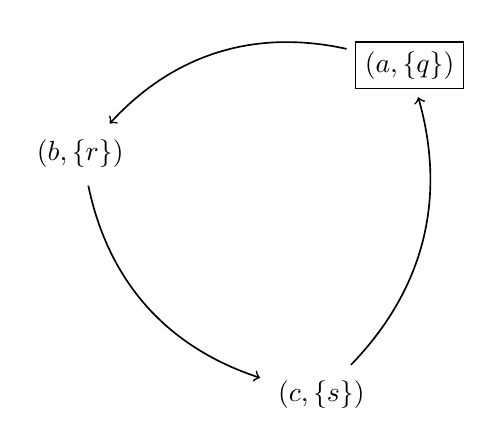
\begin{tikzpicture}[->,
         shorten >=3pt, shorten <= 3pt, 
         auto,node distance=4cm, semithick]
  \tikzstyle{state}=[draw=black, shape=rectangle]
  \tikzstyle{empt} = [draw=none,fill=none]
\begin{scope}
\node[state] (aA1) at (45:2.5) [] {$\pr{a}{\{q\}}$};
\node[empt] (aA2) at (165:2.5) {$\pr{b}{\{r\}}$};
\node[empt] (aA3) at (285:2.5) {$\pr{c}{\{s\}}$};
\path
(aA1) edge [->,bend right] node {} (aA2)
(aA2) edge [->,bend right] node {} (aA3)
(aA3) edge [->,bend right] node {} (aA1);
\end{scope}
\end{tikzpicture}
\caption{$\mathfrak{M},\pr{a}{\{q\}}\VDash \tau[\Psi]$}
   \label{fig:mod4}
\end{figure}
On the other hand, suppose there was some model $\mathfrak{N}$ such that $\mathfrak{N}, ( a, A) \VDash \tau(p)$ for all $p \in \Psi$.
This implies that $\mathfrak{N}, ( a, A) \VDash p$ for each $p \in
\Phi$.  Moreover, let $( b, B)\in\mathfrak{N}$ be such that $b \models A$ 
(one exists since by hypothesis $\mathfrak{N}, ( a, A)
\VDash \Pos p$).  By the semantics of $\tau(p)$, it is evident that
$\mathfrak{N}, ( b, B) \VDash \neg p$ and that there's a $( c, C)\in\mathfrak{N}$
such that $c \models B$ and $\mathfrak{N},( c,C )
\VDash p \wedge \Pos p$.  But then from this it must be that $a$ and
$c$ both contain exactly the same sentence letters, so $a = b$ which means that
$a \models B$ as well, since $B \subseteq
\mathcal{L}_0$ (as per the grammar restriction).  However it cannot be that
$\mathfrak{N},( a,A ) \VDash \Pos p$ since $\mathfrak{N},( a,A )
\VDash \Nec \neg p$, which follows from the assumption that $\mathfrak{N},( a,A )
\VDash \tau(p)$. 
Thus it is impossible that $\mathfrak{N},( a, A) \VDash \tau[\Phi]$. $\lightning$
\end{proof}

The above argument illustrates that while \textsc{EviL} semantics
present themselves as similar to the traditional Kripke Semantics for modal
logic, they aren't the same.  If for some reason two world-pairs
$(a,A)$ and $(b,B)$ make true the same sentence letters, then $a=b$,
and then for any $C \subseteq \mathcal{L}_0$, we have that $a \models
C$ if and only if $b \models C$. This is crucial - even though
\textsc{EviL} is modal, it has no accessibility relations; the role of
accessibility relations is instead picked up by sets of beliefs $C$. 
Since my initial design considerations for \textsc{EviL} demanded a
grammar restriction, to ensure the semantics were well-defined,
an unusual failure of compactness manifests itself.

My failure of compactness, while a fairly basic result in the model
theory of \textsc{EviL}, has far reaching consequences for the model
theory of \textsc{EviL}.  As a consequence, there is
no hope of achieving completeness using infinitary Lindenbaum
constructions that are typically employed in modal logic, such as is
done in \citep[][chapter 4]{blackburn_modal_2001}, for instance.
Hence the completeness theorem for \textsc{EviL} presented in \S\ref{army-of-darkness}
will necessarily have to be finite in nature.
%%% Local Variables: 
%%% mode: latex
%%% TeX-master: "evil_philosophy"
%%% End: 

\subsubsection{Multiple Agents}\label{multi-agent}

In this section I turn to developing the formal semantics for \tmtextsc{EviL} with a single agent.  It will be of central importance to give an account of \textsc{EviL} that is not subject to paradox.

I mentioned that the semantics previously developed in \S
gave rise to a form of {\tmem{Russell's Paradox}}.  This is due to the informal approach that I employ in presenting my intuitions.  To avoid paradoxes like this, the previous definition shall be discarded, in favor of demonstrably well-defined semantics.  This shall be achieved in two steps.

\begin{definition} Let $\mathcal{L}_0 (\Phi)$ be the language of classical propositional logic, defined by the following Backus-Naur form grammar:
\[ \phi \ {::=} \  p \in \Phi \  | \  \phi
   \rightarrow \psi \  | \  \bot \]
\end{definition}
Models for classical propositional logic can be thought of as sets $S \subseteq \Phi$; thus the truth predicate $(\models) \colons \powerset \Phi \rightarrow \mathcal{L}_0 (\Phi)
\rightarrow \textup{\textsf{bool}}${\footnote{$\ldots$ where $\textup{\textsf{bool}} := \{True, False\}$.  This is more commonly written as
$(\models) \colons \powerset \Phi \rightarrow
\textup{\textsf{bool}}^{\mathcal{L}_0 (\Phi)}$.  My notation reflects
the notation common to the typed functional programming languages
\tmtextit{Haskell} and \tmtextit{OCaml}. I will use both notations interchangeably.}} for classical propositional logic
is given recursively.  
\begin{definition}
Define $(\models)$ such that:
\begin{align*}
  S{\models}p & {\iff}p{\in}S\\
  S{\models}{\phi}{\rightarrow}{\psi} & {\iff}S{\models}{\phi}\text{ implies
  }S{\models}{\psi}\\
  S{\models}{\bot} & {\iff} False
\end{align*}
\end{definition}
Further, observe that the language $\mathcal{L}_0$ is extended by \tmtextsc{EviL}
\begin{definition} Define $\mathcal{L} (\Phi, \mathcal{A})$ by the following Backus-Naur grammar:
\[ \phi \ {::=} \  p \in \Phi \  | \  \phi
   \rightarrow \psi \  | \  \bot \  |
   \  \Box_X \phi \  | \  \boxminus_X \phi
   \  | \  \boxplus_X \phi \  | \ 
   \circlearrowleft_X \]
$\ldots$where $X \in \mathcal{A}$.
\end{definition}
%I have The two fragments  correspond to two sublogics of \textsc{EviL}. 
 \tmtextsc{EviL} models are sets $\Omega
\subseteq \powerset \Phi \times ( \mathcal{A} \rightarrow \powerset
\mathcal{L}_0 (\Phi))$.  Like classical propositional logic, semantics for
\tmtextsc{EviL} are given recursively by a predicate
\[ (\VDash) \colons \powerset ( \powerset \Phi \times ( \mathcal{A}
   \rightarrow \powerset \mathcal{L}_0 (\Phi))) \rightarrow \powerset \Phi
   \times ( \mathcal{A} \rightarrow \powerset \mathcal{L}_0 (\Phi))
   \rightarrow \mathcal{L} (\Phi, \mathcal{A}) \rightarrow
   \textup{\textsf{bool}}. \]
That is, $(\VDash)$ is a function that:
\begin{itemizedot}
  \item Takes as input:
\begin{itemizedot}
  \item An \evil model
  
  \item A pair $(a, A)$ where
  \begin{itemizedot}
    \item $a$ is a set of proposition letters
    
    \item $A:\mathcal{A}\to \mathcal{L}_0 (\Phi)$ assigns sets of formulae to agents.
  \end{itemizedot}
  \item A formula in the language $\mathcal{L} (\Phi, \mathcal{A})$
  \end{itemizedot}
  \item Gives as output: a truth value in $\textup{\textsf{bool}}$
\end{itemizedot}
I can now provide a formal definition of the semantics for $(\VDash)$:
{\footnote{Where $X \in \mathcal{A}$, I
use $A_X$ to denote $A (X)$ provided that $A \colons \mathcal{A} \rightarrow
\powerset \mathcal{L}_0 (\Phi)$}}
\begin{definition}
\begin{align*}
  {\Omega},(a,A){\VDash} p & {\iff}p{\in}a\\
  {\Omega},(a,A){\VDash} {\phi}{\rightarrow}{\psi} &
  {\iff}{\Omega},(a,A){\VDash}{\phi}\text{ implies
  }{\Omega},(a,A){\VDash}{\psi}\\
  {\Omega},(a,A){\VDash}{\bot} & {\iff} False\\
  {\Omega},(a,A){\VDash}\Box_X {\phi} & {\iff}{\forall}(b,B){\in}{\Omega}.
  ({\forall}{\psi}{\in}A_X. b{\models}{\psi})\text{ implies
  }{\Omega},(b,B){\VDash}{\phi}\\
  {\Omega},(a,A){\VDash}{\boxminus}_X{\phi} &
  {\iff}{\forall}(b,B){\in}{\Omega}. a=b\text{ and }B_X{\subseteq}A_X\text{
  implies }{\Omega},(b,B){\VDash}{\phi}\\
  {\Omega},(a,A){\VDash}{\boxplus}_X{\phi} &
  {\iff}{\forall}(b,B){\in}{\Omega}. a=b\text{ and }B_X{\supseteq}A_X\text{
  implies }{\Omega},(b,B){\VDash}{\phi}\\
  {\Omega},(a,A){\VDash}{\circlearrowleft}_X & {\iff}
  {\forall}{\psi}{\in}A_X.a{\models}{\psi}
\end{align*}
\end{definition}
These semantics are well defined, since apart from relying on the semantics
for propositional logic they may be observed to be compositional.{\footnote{In
fact, I have provided a formulation of these semantics in the same manner as
above in the computer proof assistant Isabelle/HOL(FIXME:CITATION); I shall
give my remarks on formal verification in \S(FIXME).  In the case of
Isabelle/HOL, the function $(\VDash)$ was defined inductively, and
automatically proven to be well-defined.  Specifically, the conditions given
above specify that $(\VDash)$ is determined by a \tmtextit{monotonic}
predicate over suitable tupples, and similarly for $(\models)$.  Hence the
result that $(\VDash)$ is well-defined ultimately relies on an application of
the \tmtextit{Knaster-Tarski Fixpoint Theorem} (FIXME:CITATION). Further,
since I have given an inductive definition, these recursive definitions rely
on the {\tmem{least}} fixpoint of their associated monotonic operators.}} 
Moreover, the following relationship can be observed:

\begin{lemma}
  Let $\phi \in \mathcal{L}_0 (\Phi)$.  Then:
  \[ a \models \phi \Longleftrightarrow \Omega, (a, A) \VDash \phi \]
  $\ldots$for any $\Omega$ and $A$.
\end{lemma}

\begin{proof}
  This may be seen immediately by induction on $\phi$.
\end{proof}

$\ldots$and with this, we have our central desirederatum, mirroring in Prop \ref{central-prop}:

\begin{proposition}
  Let $A$ be finite and define $$Th(\Omega) := \{ \phi \in \mathcal{L}(\Phi) \ |\ \Omega, (a,A) \VDash \phi \textup{ for all $(a,A) \in \Omega$\}}$$
\ldots then $\Omega, (a,A) \VDash \Box \phi$ if and only if $Th(\Omega) \cup A \vdash_{\text{\textsc{EviL}}} \phi$.
\end{proposition}

I shall present $\vdash_{\text{\textsc{EviL}}}$, the logical consequence turnstile for \textsc{EviL} in \S\ref{evil-axioms}.
  However, it is desirable to fist give more familiar semantics for \textsc{EviL}, so as to stress that off the shelf modal logic can be used in its investigation.
\subsubsection{Kripke Structures}\label{kripke}
The language of \textsc{EviL} is evidently modal, and in previous
sections the semantics have largely suggested that there are clear
connections to conventional Kripke semantics.  
In this section, we will demonstrate that every \textsc{EviL} model
corresponds to some highly structured Kripke model, with a minor
modification on the standard definition.  However, it will turn out
that this correspondence is one way - the class of Kripke models for
which \textsc{EviL} is strongly complete do not, in general,
possess corresponding \textsc{EviL} models.

To elucidate my intuition for understanding \textsc{EviL} models as
Kripke models, we would like to return to the visualization technique for
\textsc{EviL} models we introduced in \S\ref{contradictions}.  This
involved, roughly, thinking of the \textsc{EviL} models as 
\emph{posets} with arrows, as we first presented in 
Fig. \ref{fig:example1}.  we have given additional examples in 
Figs. \ref{fig:example2} and \ref{fig:example3}.  
In all of these depictions, the implicit relational structure of 
\textsc{EviL} models is given visual expression.  So it seems 
only natural that this graphically perceived structure
could also find formal expression.

\begin{figure}[ht]
\centering
\subfigure[A fairly simple example]{
  \includegraphics[]{evil_pictures/first_fig.pdf}
%\caption{A fairly simple example}
\label{fig:example2}
}
\subfigure[A more complex example]{
\includegraphics[]{evil_pictures/second_fig.pdf}
\label{fig:example3}
}
\caption{\textsc{EviL} model visualizations}
\end{figure}

Following the modified semantics provided in \S\ref{multi-agent}, the
developments this section will assume multiple agents.
\begin{definition}
  Let $\Phi$ be a set of letters and let $\mathcal{A}$ be a set of agents. 
  A \textbf{Kripke structure} is a state transition system $\mathbb{M}=\langle W^{\mathbb{M}}, R^{\mathbb{M}},
  \sqsubseteq^{\mathbb{M}}, \sqsupseteq^{\mathbb{M}}, V^{\mathbb{M}},
  P^{\mathbb{M}}_{\circlearrowleft} \rangle$ where\footnote{Where
    the context is clear, we shall drop $\mathbb{M}$}:
  \begin{itemizedot}
    \item $W^{\mathbb{M}}$ is a set of worlds    
    \item $R^{\mathbb{M}} : \mathcal{A} \rightarrow \powerset (W \times W)$, $\sqsubseteq^{\mathbb{M}} : \mathcal{A} \rightarrow \powerset (W \times W)$, and $\sqsupseteq^{\mathbb{M}} : \mathcal{A} \rightarrow \powerset (W \times W)$ are
    $\mathcal{A}$-indexed sets of relations\footnote{we shall abbreviate
      $R(X)$, $\sqsubseteq(X)$ and $\sqsupseteq(X)$ as $R(X)$,
      $\sqsubseteq(X)$ and $\sqsupseteq(X)$ as $R_X$, $\sqsubseteq_X$
      and $\sqsupseteq_X$ respectively.}
    \item $V : \Phi \rightarrow \powerset (W)$ is a predicate letter valuation
    \item $P_{\circlearrowleft} : \mathcal{A} \rightarrow \powerset
      (W)$ are sets of worlds indexed by agents
  \end{itemizedot}
  Let $\mathcal{K}_{\Phi, \mathcal{A}, I}$ denote the class of Kripke structures for letters $\Phi$, agents $\mathcal{A}$, and where $W \subseteq I$.
\end{definition}
Kripke semantics given by $(\Vdash) : \mathcal{K}_{\Phi, \mathcal{A}, I} \to I
\rightarrow \text{\tmtextsf{bool}}$ for these models are defined recursively
as usual, granted the exceptional behavior of $P_{\circlearrowleft}$.
\begin{definition}
  Let $\mathbbm{M}$ be in the class $\mathcal{K}_{\Phi, \mathcal{A}, I}$
  \begin{eqnarray*}
    \mathbbm{M}, w \Vdash p & \Longleftrightarrow & w \in V^{\mathbbm{M}}
    (p)\\
    \mathbbm{M}, w \Vdash \phi \rightarrow \psi & \Longleftrightarrow &
    \mathbbm{M}, w \Vdash \phi \text{ implies } \mathbbm{M}, w \Vdash \psi\\
    \mathbbm{M}, w \Vdash \bot & \Longleftrightarrow & \text{False}\\
    \mathbbm{M}, w \Vdash \Box_X \phi & \Longleftrightarrow & \forall v \in
    W^{\mathbbm{M}} . w R^{\mathbbm{M}}_X v \text{ implies } \mathbbm{M}, v
    \Vdash \phi\\
    \mathbbm{M}, w \Vdash \boxminus_X \phi & \Longleftrightarrow & \forall v
    \in W^{\mathbbm{M}} . w \sqsupseteq^{\mathbbm{M}}_X v \text{ implies }
    \mathbbm{M}, v \Vdash \phi\\
    \mathbbm{M}, w \Vdash \boxplus_X \phi & \Longleftrightarrow & \forall v
    \in W^{\mathbbm{M}} . w \sqsubseteq^{\mathbbm{M}}_X v \text{ implies }
    \mathbbm{M}, v \Vdash \phi\\
    \mathbbm{M}, w \Vdash \circlearrowleft_X & \Longleftrightarrow & w \in
    P_{\circlearrowleft}^{\mathbbm{M}} (X)
  \end{eqnarray*}
\end{definition}
Kripke structures can be observe to have a lot less structure than
\tmtextsc{EviL} models.  However, \tmtextsc{EviL} models can be understood as
Kripke structures in disguise.  To illustrate this, observe the following
lemma:
\begin{definition}[$\mho^\Omega$ Translation]
Let $\Omega$ be an \tmtextsc{EviL} model.  Define
  $\mho^{\Omega} \assign \langle \Omega, R^{\Omega},
  \sqsubseteq^{\Omega}, \sqsupseteq^{\Omega}, V^{\Omega},
  P_{\circlearrowleft}^{\Omega} \rangle$, where
  \[ \begin{array}{llll}
       \bullet & \text{$(a, A) R^{\Omega}_X (b, B) \Longleftrightarrow \forall
       \psi \in A_X .b \models \psi$} & \bullet & (a, A)
       \sqsubseteq^{\Omega}_X (b, B) \Longleftrightarrow a = b \text{ and }
       A_X \subseteq B_X\\
       \bullet & (a, A) \sqsupseteq^{\Omega}_X (b, B) \Longleftrightarrow a =
       b \text{ and } A_X \supseteq B_X & \bullet & (a, A) \in
       P_{\circlearrowleft}^{\Omega} (X) \Longleftrightarrow \forall \psi \in
       A_X .a \models \psi
     \end{array} \]
\end{definition}
\begin{lemma}
  \label{tranlemma1} For all $\Omega$ and all $(a, A) \in \Omega$,  $\Omega, (a, A) \VDash
  \phi$ if and only if $\mho^{\Omega}, (a, A) \Vdash \phi$
\end{lemma}
\begin{proof}
  This follows from a straightforward induction on $\phi$.
\end{proof}
The following summarizes the structural properties of
\tmtextsc{EviL} models, when transformed into Kripke structures:
\begin{proposition}\label{evil_models}
  For any \textsc{EviL} model $\Omega$,  $\mho^{\Omega}$ has the following
  properties{\footnote{Note that in this we have that $\{w,v\} \subseteq \powerset \Phi
      \times \powerset \mathcal{L}_0$ in the subsequent discussion}}:
  \begin{myRoman}
    \item\label{pI} $\sqsupseteq^{\Omega}_X$ is reflexive
    \item $\sqsupseteq^{\Omega}_X$ is transitive 
    \item \label{pantisym}$\sqsupseteq^{\Omega}_X$ is anti-symmetric
    \item $w \sqsupseteq^{\Omega}_X v$ if and only if $v
    \sqsubseteq^{\Omega}_X w$
    \item If $w \sqsubseteq^{\Omega}_X v$ then $w \in V (p)$ if and only if $v
    \in V (p)$
    \item \label{pV}$(R^{\Omega}_X \circ \sqsubseteq^{\Omega}_X) \subseteq
    R^{\Omega}_X \subseteq (R^{\Omega}_X \circ \sqsupseteq^{\Omega}_X)$
    \item \label{pVI} $(\sqsubseteq^{\Omega}_Y \circ R^{\Omega}_X) = R^{\Omega}_X =
    (\sqsupseteq^{\Omega}_Y \circ R^{\Omega}_X)$
    \item\label{pVII} $w \in P_{\circlearrowleft}^{\Omega} (X)$ if and only if $w
    R^{\Omega}_X w$
  \end{myRoman}
  \ldots the situation in \ref{pV} can be visualized in
  \ref{fig:commut1}, while \ref{pVI} can be split into
  Figs. \ref{fig:commut2} and \ref{fig:commut3}.
\end{proposition}
\begin{figure}[ht]
\centering
\subfigure[\ref{pV} - $(R^{\Omega}_X \circ \sqsubseteq^{\Omega}_X) \subseteq
R^{\Omega}_X$ and $R^{\Omega}_X \subseteq (R^{\Omega}_X \circ
\sqsupseteq^{\Omega}_X)$ ]{
  \includegraphics[]{commutative/commutative1.pdf}
%\caption{A fairly simple example}
\label{fig:commut1}
}
\hspace{1cm}
\subfigure[\ref{pVI} - $(\sqsubseteq^{\Omega}_Y \circ R^{\Omega}_X) \subseteq
R^{\Omega}_X$ and \ \ \ \  $R^{\Omega}_X \subseteq
(\sqsupseteq^{\Omega}_Y \circ R^{\Omega}_X)$]{
\includegraphics[]{commutative/commutative2.pdf}
\label{fig:commut2}
}
\hspace{1cm}
\subfigure[\ref{pVI} - $(\sqsupseteq^{\Omega}_Y \circ R^{\Omega}_X) \subseteq
R^{\Omega}_X $ and \ \ \ \  $R^{\Omega}_X \subseteq
(\sqsubseteq^{\Omega}_Y \circ R^{\Omega}_X)$]{
\includegraphics[]{commutative/commutative3.pdf}
\label{fig:commut3}
}
\caption{Visualizations of the relationships in Proposition \ref{evil_models}}
\end{figure}
\begin{proof}
  Everything except \ref{pV} follows directly from the definitions - so we shall only
  demonstrate $R^{\Omega}_X \subseteq R^{\Omega}_X \circ
  \sqsupseteq^{\Omega}_X$.
  
  Suppose that $(a, A) R^{\Omega}_X (b, B)$, then evidently $\forall \psi \in
  A_X .b \models \psi$. 
  Now assume that $(a, A) \sqsupseteq_X^{\Omega} (c,
  C)$.  Then we know that $A_X \supseteq C_X$.
  But then $\forall \psi \in
  C_X .b \models \psi$, so $(c, C) R^{\Omega}_X (b, B)$, which
  suffices to show the claim.
\end{proof}

\begin{definition}
A Kripke structure is called \textsc{EviL} if it makes true the
  above properties \ref{pI} through \ref{pVII} (with the exception of \ref{pantisym}, which is optional).
\end{definition}

These properties are definitive - as shall be demonstrated in \S\ref{Abstract-Completeness}, \tmtextsc{EviL} is
sound and strongly complete for \tmtextsc{EviL} models.

The Kripke semantics also serve to provide proper intuition behind
\tmtextsc{EviL} models. We think of the defined relations given as follows:
\begin{itemizedot}
  \item If $x R^{\Omega}_X y$, then at world $x$ the agent $X$ can imagine $y$
  is true, since $y$ is compatible with what the agent believes 
  \item If $x \sqsubseteq^{\Omega}_X y$, then at world $x$, agent $X$'s
  assumptions (or the experiences they are taking under consideration) are
  contained in her evidence at $y$
\end{itemizedot}
Given this perspective, the proof of \ref{pV} can be understood in the
following way - if the agent assumes fewer things, more things are imaginable,
since it's easier for a world to be incompatible with an agent's evidence.

Finally, while Prop. \ref{evil_models} presents itself as a sort of
representation lemma, the relationship between \textsc{EviL} semantics
and Kripke semantics is not reciprocal.  Not every Kripke model can be
represented as an \textsc{EviL} model.  Example
\ref{not-an-evil-model} presents an elementary example of 
this failure of representation.  It turns on the following
observation:

\begin{lemma}
  For a given \textsc{EviL} model $\mathfrak{M}$, for any
  $\{(a,A),(b,B),(c,C)\} \subseteq \mathfrak{M}$, if $a = b$ then $a
  \models C$ if and only if $b \models C$
\end{lemma}
\begin{proof}
  This is an elementary result in the semantics of propositional logic.
\end{proof}

\begin{example}\label{not-an-evil-model}
Consider a single agent \textsc{EviL} Kripke structure $\mathbb{M}:=\langle W, R,
  \sqsubseteq, \sqsupseteq, V, P \rangle$ where
\begin{bul}
  \item $W := \{w,v\}$
  \item $R := \{(w,v)\}$
  \item $ \sqsubseteq := \sqsupseteq := \{(w,w),(v,v)\}$
  \item $V(p) := \varnothing$ for all $p\in \Phi$
  \item $P := \varnothing$
\end{bul}
\ldots this structure is indicated in Fig. \ref{fig:notevil}.  No
\textsc{EviL} model corresponds to $\mathbb{M}$.
%\end{lemma}
\begin{figure}[ht]
\centering
  \includegraphics[]{evil_pictures/third_fig.pdf}
%\caption{A fairly simple example}
\label{fig:notevil}
\caption{$\mathbb{M}$ is a Kripke Structure with no \textsc{EviL} representation}
\end{figure}
%\begin{proof}

Observe that the above model makes true the following:

\begin{align}
  \mathbb{M},w & \Vdash \Pos \top \label{notevil:eq1}\\
  \mathbb{M},w & \Vdash \Nec \neg p \textup{ for all $p \in
    \Phi$} \label{notevil:eq4} \\
  \mathbb{M},w & \Vdash \neg p \textup{ for all $p \in \Phi$} \label{notevil:eq2} \\
  \mathbb{M},w & \Vdash \neg \Pos \Pos \top \label{notevil:eq3} 
\end{align}

Armed with these observations, we can assert that it is impossible for
there to be an \textsc{EviL} structure $\mathfrak{M}$ with a world
$(a,A)$ such that $\mathbb{M},w \Vdash \phi$ if and only if
$\mathfrak{M}, (a,A) \VDash \phi$.

For suppose there were, then we could deduce the following facts, using
the observations above:
\begin{mynum}
\item\label{notevil:1} From \eqref{notevil:eq1}, there must be some pair $(b,B)
   \in \mathfrak{M}$ such that $b\models A$.  Hence, $A$ must be
   \emph{consistent}.
\item From \eqref{notevil:eq4}, we know that for the $b$ mentioned in
  \ref{notevil:1}, it must be that $b = \varnothing$ -- this is a
  direct consequence of Lemma \ref{truthiness}, the Truthiness Lemma.
 \item From \eqref{notevil:eq2}, evidently $a = \varnothing$
  \item From \eqref{notevil:eq3}, it must be
    that $a \nmodels A$, since otherwise we would have
    $\mathfrak{M},(a,A) \VDash \Pos \Pos \top$
\end{mynum}
This is absurd... since $a = b = \varnothing$ and $b \models A$
then it must be that $a \models A$. $\lightning$
%\end{proof}
\end{example}

The above one way correspondence is inconvenient - it means that while
\textsc{EviL} only enjoys some features from modal logic, it is denied
others.  Despite this, \textsc{EviL} enjoys \emph{most} of the
benefits of basic modal logic.  Furthermore, even though \textsc{EviL}
is quite formal in nature, it might rightly be considered an
application  of traditional modal logic rather than a novel logic
in of itself.   The novelty of \textsc{EviL} is that it presents semantics
that automatically connect truth and derivability (as expressed in
Theorem \ref{theorem-theorem}, the Theorem Theorem).

%%% Local Variables: 
%%% mode: latex
%%% TeX-master: "evil_philosophy"
%%% End: 

%% \documentclass{letter}
% \usepackage{geometry,amsmath,amssymb,bbm}
% \geometry{letterpaper}
% 
% %%%%%%%%%% Start TeXmacs macros
% \newcommand{\tmop}[1]{\ensuremath{\operatorname{#1}}}
% \newcommand{\tmtextit}[1]{{\itshape{#1}}}
% \newcommand{\tmtextsc}[1]{{\scshape{#1}}}
% \newenvironment{itemizedot}{\begin{itemize} \renewcommand{\labelitemi}{$\bullet$}\renewcommand{\labelitemii}{$\bullet$}\renewcommand{\labelitemiii}{$\bullet$}\renewcommand{\labelitemiv}{$\bullet$}}{\end{itemize}}
% %%%%%%%%%% End TeXmacs macros
% 
% \begin{document}

These properties are definitive - as we shall demonstrate, \tmtextsc{EviL} is
sound and weakly complete for \tmtextsc{EviL} models.

The Kripke semantics also serve to \ provide proper intuition behind
\tmtextsc{EviL} models. \ I think of the defined relations given as follows:
\begin{itemizedot}
  \item If $x R^{\Omega}_X y$, then at world $x$ the agent $X$ can imagine $y$
  is true, since $y$ is compatible with what the agent believes
  
  \item If $x \sqsubseteq^{\Omega}_X y$, then at world $x$, agent $X$'s
  assumptions (or the experiences they are taking under consideration) are
  contained in her evidence at $y$
\end{itemizedot}
Given this perspective, the proof of \ref{pV} can be understood in the
following way - if the agent assumes fewer things, more things are imaginable,
since it's easier for a world to be incompatible with an agent's evidence.

Another expression of the same idea as above is as follows. \ For a given
Kripke structure $\mathbbm{M}$, define two operators $Mod^{\mathbbm{M}}
: \powerset  \mathcal{L} (\Phi, \mathcal{A}) \rightarrow \powerset
(W^{\mathbbm{M}})$ and $Th^{\mathbbm{M}} : \powerset
(W^{\mathbbm{M}}) \rightarrow \powerset \mathcal{L} (\Phi, \mathcal{A})$:

\begin{align*}
  Mod^{{\mathbbm{M}}}({\Delta}) &
  =\{x{\in}W{\ }|{\ }{\forall}{\psi}{\in}{\Delta}.
  {\mathbbm{M}},x{\Vdash}{\psi}\}\\
  Th^{{\mathbbm{M}}}({\nabla}) & =\{{\psi}{\in}\mathcal{L}({\Phi},
  \mathcal{A}){\ }|{\ }{\forall}x{\in}{\nabla}.
  {\mathbbm{M}},x{\Vdash}{\psi}\}
\end{align*}

The following relationship holds, where $\Delta \in \powerset  \mathcal{L}
(\Phi, \mathcal{A})$ and $\nabla \in \powerset (W^{\mathbbm{M}})$:
\[ \nabla \subseteq Mod^{\mathbbm{M}} (\Delta) \text{ if and only if }
   \Delta \subseteq Th^{\mathbbm{M}} (\nabla) \]
$\ldots$hence we these two operations form what is refered an
\tmtextit{antitone Galois connection}, between the lattice $\powerset
(W^{\mathbbm{M}})$ and the lattice $\powerset \mathcal{L} (\Phi,
\mathcal{A})$. \ It follows from the theory of Galois connections (FIXME) that
the following two properties hold:
\begin{itemizedot}
  \item If $\nabla \supseteq \nabla'$ then $Th^{\mathbbm{M}} (\nabla)
  \subseteq Th^{\mathbbm{M}} (\nabla')$
  
  \item If $\Delta \supseteq \Delta'$ then $Mod^{\mathbbm{M}} (\Delta)
  \subseteq Mod^{\mathbbm{M}} (\Delta')$
\end{itemizedot}
We can see that (\ref{pV}) follows from the second of these two properties. \
To see this, assume that $(a, A) \sqsupseteq_X^{\Omega} (b, B)$, hence $A_X
\supseteq B_X$ and thus $Mod^{\Omega} (A_X) \subseteq
Mod^{\Omega} (B_X)$. \ But it follows from semantics of \tmtextsc{EviL}
we have that $(c, C) \in Mod^{\Omega} (A_X)$ if and only if $(a, A)
R^{\Omega}_X (c, C)$, and likewise for $B_X$. \ Hence if $(a, A) R^{\Omega}_X
(c, C)$ then $(b, B) R^{\Omega}_X (c, C)$.

% \end{document}
\subsection{\textsc{EviL} Completeness}\label{army-of-darkness}
\subsubsection{Axiom Systems}\label{evil-axioms}
In this section, we shall present the axiom system which represents
the validities of \textsc{EviL} semantics as provided in . 

Table \ref{table:axioms}, provides a Hilbert-style axiom system for \textsc{EviL}.  In addition to giving each axiom, we have also provided our own philosophical reading of what each axiom says.  One unusual feature of this logic is that it is not \emph{normal}, that is it is not closed under variable substitution.

\begin{table}
\newcounter{rownum}
\setcounter{rownum}{0}
\newcounter{rownum2}
\setcounter{rownum2}{0}
\begin{tabularx}{\linewidth}{|cl>{\it}X|}
\hline
(\refstepcounter{rownum}\arabic{rownum}) & $\vdash \phi \to \psi \to \phi$ & \multirow{3}{*}{Axioms for basic propositional logic} \\
(\arabic{rownum}) & $\vdash (\phi \to \psi \to \chi) \to (\phi \to \psi) \to \phi \to \chi$ &  \\
(\refstepcounter{rownum}\arabic{rownum}) & $\vdash (\neg \phi \to \neg \psi) \to \psi \to \phi$ &  \\[6pt]
(\refstepcounter{rownum}\arabic{rownum}\label{reflAx})
 & $\vdash \BBI_X \phi \to \phi$ & If $\phi$ holds under any further evidence $X$ considers, then $\phi$ holds simpliciter, since considering no additional evidence is trivially considering further evidence \\[6pt]
(\refstepcounter{rownum}\arabic{rownum})\label{transAx} & $\vdash \BBI_X \phi \to \BBI_X \BBI_X \phi$ & If $\phi$ holds under any further evidence $X$ considers, then $\phi$ holds whenever $X$ considers even further evidence beyond that \\[6pt]
(\refstepcounter{rownum}\arabic{rownum})\label{letterAx1} & $\vdash p \to \BB_X p$ & \multirow{2}{8.5cm}{Changing one's mind does not bear on matters of fact}\\
(\refstepcounter{rownum}\arabic{rownum})\label{letterAx2} & $\vdash p \to \BBI_X p$ & \\[6pt]
(\refstepcounter{rownum}\arabic{rownum})\label{downConceive} & $\vdash \Pos_X \phi \to \BB_X \Pos_X \phi$ & The more evidence $X$ discards, the freer her imagination can run \\[6pt]
(\refstepcounter{rownum}\arabic{rownum})\label{islandDown} & $\vdash \Nec_X \phi \to \Nec_X \BB_Y \phi$ &  \multirow{2}{8.5cm}{If $X$ believes a proposition, she believes it regardless of what anyone else thinks} \\
(\refstepcounter{rownum}\arabic{rownum})\label{islandUp} & $\vdash \Nec_X \phi \to \Nec_X \BBI_Y \phi$ & \\[6pt]
(\refstepcounter{rownum}\arabic{rownum})\label{soundness} & $\vdash \PP_X \to \Nec_X \phi \to \phi$ & If $X$'s premises are sound, then her logical conclusion are correct \\[6pt]
(\refstepcounter{rownum}\arabic{rownum})\label{downsound} & $\vdash \PP_X \to \BB_X \PP_X $ & If $X$'s premises are sound then any subset will be sound as well \\[6pt]
(\refstepcounter{rownum}\arabic{rownum})\label{reverseAx1} & $\vdash \phi \to \BB_X \DDI_X \phi$ &
\multirow{2}{8.5cm}{Embracing evidence is the inverse of discarding evidence} 
\\
(\refstepcounter{rownum}\arabic{rownum})\label{reverseAx2} & $\vdash \phi \to \BBI_X \DD_X \phi$ & \\[6pt]
(\refstepcounter{rownum}\arabic{rownum}) & $\vdash \Nec_X (\phi \to \psi) \to \Nec_X \phi \to \Nec_X \psi$ &
\multirow{3}{8.5cm}{Variations on axiom $K$}
\\
(\refstepcounter{rownum}\arabic{rownum}) & $\vdash \BB_X (\phi \to \psi) \to \BB_X \phi \to \BB_X \psi$ & \\
(\refstepcounter{rownum}\arabic{rownum}) & $\vdash \BBI_X (\phi \to \psi) \to \BBI_X \phi \to \BBI_X \psi$ & \\[6pt]
(\refstepcounter{rownum2}\Roman{rownum2}) & 
 $\AxiomC{$\vdash \phi \to \psi$}
\AxiomC{$\vdash \phi$}
\BinaryInfC{$\vdash \psi$}
\DisplayProof$ & Modus Ponens\\[10pt]
(\refstepcounter{rownum2}\Roman{rownum2}) & 
 $\AxiomC{$\vdash \phi$}
\UnaryInfC{$\vdash \Box_X \phi$}
\DisplayProof$ & \multirow{3}{8.5cm}{Variations on necessitation}\\
(\refstepcounter{rownum2}\Roman{rownum2}) \label{BMnec}& 
 $\AxiomC{$\vdash \phi$}
\UnaryInfC{$\vdash \BB_X \phi$}
\DisplayProof$ &  \\
(\refstepcounter{rownum2}\Roman{rownum2}) &
 $\AxiomC{$\vdash \phi$}
\UnaryInfC{$\vdash \BBI_X \phi$}
\DisplayProof$ & \\[10pt]
\hline
\end{tabularx}
\caption{A Hilbert style axiom system for \textsc{EviL}}
\label{table:axioms}
\end{table}


%%% Local Variables: 
%%% mode: latex
%%% TeX-master: "../evil_philosophy"
%%% End: 


This logic makes true a variety of relationships between the various
modalities, which are given in the following lemma:
\begin{lemma}\label{equivs}
We have the following provable equivalences:
\begin{eqnarray*} \vdash \Nec_X \phi \IFF \BB_X \Nec_X \phi & \hspace{1cm} \vdash \Nec_X \phi \IFF \Nec_X \BB_Y \phi \hspace{1cm}  & \vdash \Nec_X \phi \IFF \Nec_X \BBI_Y \phi \\
 \vdash \BB_X \phi \IFF \BB_X \BB_X \phi & \vdash \BBI_X \phi \IFF \BBI_X \BBI_X \phi & \vdash \PP_X \IFF \BB_X \PP_X\end{eqnarray*}
%&\vdash \PP_X \IFF \DDI_X \PP_X \\
%&\vdash \phi \IFF \psi \textup{ implies } \vdash \chi \IFF \chi[\phi/\psi]
%\end{eqnarray*}
%\ldots where $\chi[\phi/\psi]$ is the same as $\chi$ but every occurrence of $\phi$ as a subformula is replaced by $\psi$.
%$\hfill\dashv$
\end{lemma}

In addition to the main system presented above, it can be understood to contain two subsystems, corresponding to two fragments of the main grammar:
\begin{definition}
Define $\mathcal{L}^\boxminus (\Phi, \mathcal{A})$ as the fragment:
\[ \phi \ {::=} \  p \in \Phi \  | \  \phi
   \rightarrow \psi \  | \  \bot \  |
   \  \Box_X \phi \  | \  \boxminus_X \phi
%   \  | \  \boxplus_X \phi
 \  | \ 
   \circlearrowleft_X \]

And define $\mathcal{L}^\boxplus (\Phi, \mathcal{A})$ as the fragment:
%Define $\mathcal{L}^\boxminus (\Phi, \mathcal{A})$ as the fragment:
\[ \phi \ {::=} \  p \in \Phi \  | \  \phi
   \rightarrow \psi \  | \  \bot \  |
   \  \Box_X \phi 
%\  | \  \boxminus_X \phi
   \  | \  \boxplus_X \phi
 \  | \ 
   \circlearrowleft_X \]
\end{definition}

Table \ref{table:axiomsII} gives the axioms systems for these two fragments.  For now, we shall observe that \textsc{EviL} extends \textsc{EviL}$^\BM$ and \textsc{EviL}$^\BP$.  In \S\ref{conservative-extension} we shall make this precise. 
\begin{table}
\begin{minipage}[b]{0.5\linewidth}
\centering
%\newcounter{rownum}
\setcounter{rownum}{0}
%\newcounter{rownum2}
\setcounter{rownum2}{0}
\begin{tabular}{|ll|}
\hline
  (\addtocounter{rownum}{1}\arabic{rownum})&$ \vdash \phi \rightarrow \psi \rightarrow \phi$\\
  (\addtocounter{rownum}{1}\arabic{rownum})&$ \vdash (\phi \rightarrow \psi \rightarrow \chi) \rightarrow (\phi
  \rightarrow \psi) \rightarrow \phi \rightarrow \chi$\\
  (\addtocounter{rownum}{1}\arabic{rownum})&$ \vdash (\neg \phi \rightarrow \neg \psi) \rightarrow \psi \rightarrow
  \phi$\\
  (\addtocounter{rownum}{1}\arabic{rownum})&$ \vdash \boxminus_X \phi \rightarrow \phi$\\
  (\addtocounter{rownum}{1}\arabic{rownum})&$ \vdash \boxminus_X \phi \rightarrow \boxminus_X \boxminus_X \phi$\\
  (\addtocounter{rownum}{1}\arabic{rownum})&$ \vdash p \rightarrow \boxminus_X p$\\
  (\addtocounter{rownum}{1}\arabic{rownum})&$ \vdash \neg p \rightarrow \boxminus_X \neg p$\\
  (\addtocounter{rownum}{1}\arabic{rownum})&$ \vdash \diamondsuit_X \phi \rightarrow \boxminus_X \diamondsuit_X \phi$\\
  (\addtocounter{rownum}{1}\arabic{rownum})&$ \vdash \Box_X \phi \rightarrow \Box_X \boxminus_Y \phi$\\
  (\addtocounter{rownum}{1}\arabic{rownum})&$ \vdash \phi \rightarrow \boxminus_X (\circlearrowleft_X \rightarrow
  \diamondsuit_X \phi)$\\
  (\addtocounter{rownum}{1}\arabic{rownum})&$ \vdash \circlearrowleft_X \rightarrow \boxminus_X \circlearrowleft_X$\\
  (\addtocounter{rownum}{1}\arabic{rownum})&$ \vdash \Box_X (\phi \rightarrow \psi) \rightarrow \Box_X \phi \rightarrow
  \Box_X \psi$\\
  (\addtocounter{rownum}{1}\arabic{rownum})&$ \vdash \boxminus_X (\phi \rightarrow \psi) \rightarrow \boxminus_X \phi
  \rightarrow \boxminus_X \psi$\\
(\addtocounter{rownum2}{1}\Roman{rownum2}) & 
 $\AxiomC{$\vdash \phi \to \psi$}
\AxiomC{$\vdash \phi$}
\BinaryInfC{$\vdash \psi$}
\DisplayProof$ \\ %& Modus Ponens\\[10pt]
(\addtocounter{rownum2}{1}\Roman{rownum2}) & 
 $\AxiomC{$\vdash \phi$}
\UnaryInfC{$\vdash \Box_X \phi$}
\DisplayProof$ \\ %& \multirow{3}{8.5cm}{Variations on necessitation}\\
(\addtocounter{rownum2}{1}\Roman{rownum2}) & 
 $\AxiomC{$\vdash \phi$}
\UnaryInfC{$\vdash \BB_X \phi$}
\DisplayProof$   \\
% (\addtocounter{rownum2}{1}\Roman{rownum2}) &
%  $\AxiomC{$\vdash \phi$}
% \UnaryInfC{$\vdash \BBI_X \phi$}
% \DisplayProof$  \\% [10pt]
\hline
\end{tabular}
\end{minipage}
\hspace{0.5cm}
\begin{minipage}[b]{0.5\linewidth}
 \centering
%\newcounter{rownum}
\setcounter{rownum}{0}
%\newcounter{rownum2}
\setcounter{rownum2}{0}
\begin{tabular}{|ll|}
\hline
  (\addtocounter{rownum}{1}\arabic{rownum})&$ \vdash \phi \rightarrow \psi \rightarrow \phi$\\
  (\addtocounter{rownum}{1}\arabic{rownum})&$ \vdash (\phi \rightarrow \psi \rightarrow \chi) \rightarrow (\phi
  \rightarrow \psi) \rightarrow \phi \rightarrow \chi$\\
  (\addtocounter{rownum}{1}\arabic{rownum})&$ \vdash (\neg \phi \rightarrow \neg \psi) \rightarrow \psi \rightarrow
  \phi$\\
  (\addtocounter{rownum}{1}\arabic{rownum})&$ \vdash \boxplus_X \phi \rightarrow \phi$\\
  (\addtocounter{rownum}{1}\arabic{rownum})&$ \vdash \boxplus_X \phi \rightarrow \boxplus_X \boxplus_X \phi$\\
  (\addtocounter{rownum}{1}\arabic{rownum})&$ \vdash p \rightarrow \boxplus_X p$\\
  (\addtocounter{rownum}{1}\arabic{rownum})&$ \vdash \neg p \rightarrow \boxplus_X \neg p$\\
  (\addtocounter{rownum}{1}\arabic{rownum})&$ \vdash \Box_X \phi \rightarrow \boxplus_X \Box_X \phi$\\
  (\addtocounter{rownum}{1}\arabic{rownum})&$ \vdash \Box_X \phi \rightarrow \Box_X \boxplus_Y \phi$\\
  (\addtocounter{rownum}{1}\arabic{rownum})&$ \vdash \phi \rightarrow \boxplus_X (\circlearrowleft_X \rightarrow
  \diamondsuit_X \phi)$\\
  (\addtocounter{rownum}{1}\arabic{rownum})&$ \vdash \neg \circlearrowleft_X \rightarrow \boxplus_X \neg
  \circlearrowleft_X$\\
  (\addtocounter{rownum}{1}\arabic{rownum})&$ \vdash \Box_X (\phi \rightarrow \psi) \rightarrow \Box_X \phi \rightarrow
  \Box_X \psi$\\
  (\addtocounter{rownum}{1}\arabic{rownum})&$ \vdash \boxplus_X (\phi \rightarrow \psi) \rightarrow \boxplus_X \phi
  \rightarrow \boxplus_X \psi$\\
(\addtocounter{rownum2}{1}\Roman{rownum2}) & 
 $\AxiomC{$\vdash \phi \to \psi$}
\AxiomC{$\vdash \phi$}
\BinaryInfC{$\vdash \psi$}
\DisplayProof$ \\ %& Modus Ponens\\[10pt]
(\addtocounter{rownum2}{1}\Roman{rownum2}) & 
 $\AxiomC{$\vdash \phi$}
\UnaryInfC{$\vdash \Box_X \phi$}
\DisplayProof$ \\ %& \multirow{3}{8.5cm}{Variations on necessitation}\\
% (\addtocounter{rownum2}{1}\Roman{rownum2}) & 
%  $\AxiomC{$\vdash \phi$}
% \UnaryInfC{$\vdash \BB_X \phi$}
% \DisplayProof$   \\
(\addtocounter{rownum2}{1}\Roman{rownum2}) &
 $\AxiomC{$\vdash \phi$}
\UnaryInfC{$\vdash \BBI_X \phi$}
\DisplayProof$  \\% [10pt]
\hline
\end{tabular}
\end{minipage}
\caption{Axiom system \textsc{EviL}$^\BM$ and \textsc{EviL}$^\BP$ respectively}
\label{table:axiomsII}
\end{table}

%%% Local Variables: 
%%% mode: latex
%%% TeX-master: "evil_philosophy"
%%% End: 

%\subsection{Axiomatics}
%\subsection{Soundness \& Completeness}

%In the subsequent discussion, let the Tarski predicate $(\Vdash)$ denote the usual Kripke semantics for the language $\mathcal{L}(\Phi)$ for structures $\langle W, V, P_X, R_{\Box_X}, R_{\BB_X}, R_{\BBI_X}\ra$.  The only unconventional thing we shall doe is to declare $P_X \subseteq W$ and $\mathbb{M},w \vdash \PP_X$ if and only if $w \in P_X$.
%In the subsequent discussion we shall employ the Fraktur typeface (such as $\mathfrak{M}$) to denote models in \textsc{EviL} semantics and the blackboard typeface (such as $\mathbb{M}$) to denote models in Kripke semantics.

From the definitions so far the following can be seen to hold:
\begin{lemma}[Soundness]
If $\vdash \phi$ then for any model $\mathfrak{M}$ and any $(a,A) \in \mathfrak{M}$ we have that $\mathfrak{M},(a,A) \models \phi$ 
\end{lemma}

The proof of the converse, that is \emph{completeness}, proceeds by a three stage construction:
\begin{bul}
\item The first step is to construct a Kripke model $\Cross^\phi$ consisting of finite maximally consistent sets of formulae related to $\phi$ where $\Cross^\phi,w \nVdash \phi$ for some world $w \in W^{\Cross^\phi}$. This model will be shown to make true nine properties.
\item The second step is to construct a model ${\iCross^{\Cross^\phi}}$ which is bisimular to $\Cross^\phi$. This model also makes true these nine properties as well as an additional tenth property.
\item The final third step is to construct an \textsc{EviL} model ${\ipent^{\iCross^{\Cross^\phi}}_\phi}$.
I shall then show that for each $w \in W^{\iCross^{\Cross^\phi}}$ there is a corresponding $(a,A) \in \ipent^{\iCross^{\Cross^\phi}}_\phi$ such that ${\iCross^{\Cross^\phi}}, w \Vdash \psi$ if and only if ${\ipent^{\iCross^{\Cross^\phi}}_\phi},(a,A) \models \psi$ for all subformulae $\psi$ of $\phi$.
\end{bul}
These three steps together suffice to prove completeness.  I shall now proceed to demonstrate these constructions.
\subsubsection{Subformula Model Construction}
In this section we provide definitions and lemmas related to the subformula construction $\Cross^\phi$.  I consciously imitate \citet{boolos_logic_1995} in my approach, as well as the ``Fischer-Ladner Closure'' used in the completeness theorem of PDL \citep{blackburn_modal_2001}.
\begin{mydef}
\begin{eqnarray*}
\sim \phi := \begin{cases} \psi &\textup{ if $\phi = \neg\psi$} \\ \neg \phi & \textup{ o/w} \end{cases} &
\hspace{1cm} \pBB_X \phi := \begin{cases} \phi &\textup{ if $\phi = \BB_X \psi$} \\ \BB_X \phi & \textup{ o/w} \end{cases} \hspace{1cm} &
\pBBI_X \phi := \begin{cases} \phi &\textup{ if $\phi = \BBI_X \psi$} \\ \BBI_X \phi & \textup{ o/w} \end{cases}
\end{eqnarray*}
\end{mydef}
\begin{lemma}\label{equivs2} By Lemma \ref{equivs} we have
\begin{eqnarray*} 
\vdash \sim \phi \IFF \neg \phi &
\hspace{1cm} \vdash \pBB_X \phi \IFF \BB_X \phi \hspace{1cm} &
\vdash \pBBI_X \phi \IFF \BBI_X \phi
\end{eqnarray*}
\ldots moreover \ldots 
\begin{align*}
\pBB_X \phi = \pBB_X\pBB_X \phi & & \pBBI_X\phi = \pBBI_X \pBBI_X \phi \hfill
\end{align*}
\end{lemma}
\begin{mydef} Let $\delta(\phi) \subseteq \mathcal{A}$ be the set of agents that occur in $\phi$\footnote{In natural language, we read $\delta(\phi)$ as ``the dudes mentioned by $\phi$.''} \end{mydef}
\begin{mydef}Define $\Sigma( \Delta,\phi)$ using primitive recursion as follows:
\begin{tabbing}$\Sigma(\Delta,p) :=  \{ p, \neg p, \bot, \neg\bot \} \cup \bigcup\{ \{ \BB_X p, \neg\BB_X p, \BBI_X p, \neg\BBI_X p\} \ |\ X \in \Delta \}$ \\
$\Sigma(\Delta,\bot) := \{ \bot, \neg\bot \}$ \\
$\Sigma(\Delta,\PP_X) := \{ \PP_X, \neg\PP_X, \BB_X \PP_X, \neg \BB_X \PP_X, \bot, \neg\bot \}$ \\
$\Sigma(\Delta,\phi\to\psi) := \{ \phi\to\psi,\neg(\phi\to\psi) \} \cup \Sigma(\Delta,\phi) \cup \Sigma(\Delta,\psi)$ \\
$\Sigma(\Delta,\Nec_X \phi) :=$ \= $\{ \Nec_X \phi, \neg \Nec_X \phi, \BBI_X \Nec_X \phi, \neg\BBI_X\Nec_X \phi \}$ \\
\> $\cup \bigcup\{\{\Nec_X \pBB_Y \phi, \neg\Nec_X \pBB_Y \phi, \Nec_X \pBBI_Y \phi, \neg\Nec_X \pBBI_Y \phi, \pBB_Y \phi, \neg \pBB_Y \phi, \pBBI_Y \phi, \neg\pBBI_Y \phi\}\ |\ Y \in \Delta \}$ \\
\> $ \cup \Sigma(\Delta,\phi)$\\
$\Sigma(\Delta,\BB_X \phi) := \{ \BB_X \phi, \neg\BB_X \phi\} \cup \Sigma(\Delta,\phi)$ \\
$\Sigma(\Delta,\BBI_X \phi) := \{ \BBI_X \phi, \neg\BBI_X \phi\} \cup \Sigma(\Delta,\phi)$
\end{tabbing}
\end{mydef}
\begin{lemma}\label{inclusions}
$\Sigma(\delta(\phi),\phi)$ is finite.  Moreover, we have the following:
\begin{bul}
	\item If $\psi \in \Sigma(\delta(\phi),\phi)$ then $\sim \psi \in \Sigma(\delta(\phi),\phi)$
	\item If $\psi \in \Sigma(\delta(\phi),\phi)$ and $\chi$ is a subformula of $\psi$, then $\chi \in \Sigma(\delta(\phi),\phi)$
	\item If $\BB_X \phi \in \Sigma(\delta(\phi),\phi)$ then $\pBB_X \phi \in \Sigma(\delta(\phi),\phi)$
	\item If $\BBI_X \phi \in \Sigma(\delta(\phi),\phi)$ then $\pBBI_X \phi \in \Sigma(\delta(\phi),\phi)$
\end{bul}
\end{lemma}
\begin{mydef}Let $At(\Psi)$ denote the maximally consistent subsets of $\Psi$
\end{mydef}
\begin{lemma}[Lindenbaum Lemma]If $\Gamma \nvdash \phi$ and $\Gamma\subseteq \Sigma(\delta(\phi),\phi)$, then there is a $\Gamma' \in At(\Sigma(\delta(\phi),\phi))$ such that $\Gamma \subseteq \Gamma'$ and $\Gamma' \nvdash \phi$
\end{lemma}
\begin{mydef}Define $\Cross^\phi := \langle W^{\Cross^\phi}, V^{\Cross^\phi}, P^{\Cross^\phi}_X, R^{\Cross^\phi}_{\Nec_X}, R^{\Cross^\phi}_{\BB_X}, R^{\Cross^\phi}_{\BBI_X}\ra$ where:
\begin{tabbing}
$W^{\Cross^\phi} := At(\Sigma(\delta(\phi),\phi))$ \\
$V^{\Cross^\phi}(p) := \{ w \in W^{\Cross^\phi}\ |\ p \in w \}$ \\
$P^{\Cross^\phi}_X := \{ w \in W^{\Cross^\phi}\ |\ \PP_X \in w \} \cup \{ w\in W^{\Cross^\phi} \ | \ X \nin \delta(A)\}$ \\
$R^{\Cross^\phi}_{\Nec_X} := \{(w,v) \in W^{\Cross^\phi} \times W^{\Cross^\phi}\ |\ \{ \psi\ |\ \Box_X \psi \in w\} \subseteq v \}$\\
$R^{\Cross^\phi}_{\BB_X} := \{(w,v) \in W^{\Cross^\phi} \times W^{\Cross^\phi}\ |$\=$\ \bigcup \{ \{\psi,\pBB_X \psi\}\ |\ \pBB_X \psi \in w\} \subseteq v \wedge \bigcup\{ \{\psi,\pBBI_X \psi\} \ |\ \pBBI_X \psi \in v\} \subseteq w \}$ \\
$R^{\Cross^\phi}_{\BBI_X} := \{(v,w) \in W^{\Cross^\phi} \times W^{\Cross^\phi}\ |$\=$\ \bigcup \{ \{\psi,\pBB_X \psi\}\ |\ \pBB_X \psi \in w\} \subseteq v \wedge \bigcup\{ \{\psi,\pBBI_X \psi\} \ |\ \pBBI_X \psi \in v\} \subseteq w \}$
\end{tabbing}
\end{mydef}
\begin{lemma}[Truth Lemma]\label{truth}
For any subformula $\psi \in \Sigma(\delta(\phi),\phi)$ and any $w \in W^{\Cross^\phi}$, we have that $\Cross^\phi, w \Vdash \psi$ if and only if $\psi \in w$
\end{lemma}
\begin{proof} The proof proceeds by induction on $\psi$.  Most of the steps are routine, with the exception of the right to left directions for the boxes.

I shall demonstrate the right to left direction for $\BB_X$.  Assume that $\BB_X \psi \nin w$, then $w \nvdash \BB_X \psi$.  By Lemma \ref{equivs2} this is true if and only if $w \nvdash \pBB_X \psi$.  Now abbreviate:
\begin{align*}
A := & \bigcup \{ \{\chi,\pBB_X \chi\}\ |\ \pBB_X \chi \in w \}\\
B := & \{ \sim \pBBI_X \chi \ | \ \pBBI_X \chi \in \Sigma(\delta(\phi),\phi) \wedge \sim\chi \in w \}
\end{align*}
Now suppose towards a contradiction that $\{\sim \psi\} \cup A \cup B \vdash \bot$.  Then $A \cup B \vdash \psi$, and furthermore by Lemma \ref{equivs2} and rule (III) from the axioms we have that $\pBB_X A \cup \pBB_X B \vdash \pBB_X \psi$.\footnote{Here $\pBB_X S$ is shorthand for $\{ \pBB_X \chi \ |\ \chi \in S\}$.} But then let 
\begin{align*}
A' := & \{ \pBB_X \chi\ |\ \pBB_X \chi \in w \}\\
B' := & \{ \sim \chi \ | \  \sim\chi \in w \}
\end{align*}
Since $\pBB_X \pBB_X \chi = \pBB_X \chi$ by Lemma \ref{equivs2}, we have $A' = \pBB_X A$.  Moreover, by Lemma \ref{equivs2}, axiom 13, and classical logic we can see that
\[ \vdash \sim \chi \to \pBB_X \sim \pBBI_X \psi \]
Thus for every $\beta \in \pBB_X B$ we have that $B' \vdash \beta$.  Hence by $n$ applications of the Cut rule we can arrive at 
\[ A' \cup B' \vdash \pBB_X \chi \]
However, evidently $A' \cup B' \subseteq w$, hence $w \vdash \pBB_X \psi$, which contradicts what has been stipulated. $\lightning$

Hence it must be that $\{\sim \psi\} \cup A \cup B \nvdash \bot$.  In addition, from the fact that $w \subseteq \Sigma(\delta(\phi),\phi)$ with Lemma  \ref{inclusions} and the hypothesis we have that $\{\sim \psi\} \cup A \cup B \subseteq \Sigma(\delta(\phi),\phi)$.  Hence by the Lindenbaum Lemma we have that there is some $v \in At(\Sigma(\delta(\phi),\phi))$ such that $\{\sim \psi\} \cup A \cup B \subseteq v$.  By the inductive hypothesis we have that $\Cross^\phi, v \nVdash \psi$.

To complete the argument, we have to show that $w R^{\Cross^\phi}_{\BB_X} v$.  Since $A \subseteq v$ we just need to check that $\bigcup\{ \{\psi,\pBBI_X \psi\} \ |\ \pBBI_X \psi \in v\} \subseteq w$.  Suppose that $\pBBI_X \psi \in v$ but $\psi \nin w$.  Since $w$ is maximally consistent we have then that $\nin \psi \in w$.  Thus $\sim \pBBI_X \psi \in v$, which contradicts that $v$ is consistent. $\lightning$  Now suppose that $\pBBI_X \psi \in v$ but $\pBBI_X \psi \nin w$, hence $\sim \pBBI_X \psi \in w$ and thus $\sim \pBBI_X \pBBI_X \psi \in v$.  However we know from Lemma \ref{equivs2} that $\pBBI_X \pBBI_X \psi = \pBBI_X \psi$, which once again implies that $v$ is inconsistent. $\lightning$
\end{proof}

\begin{lemma}[$\Cross^\phi$ is Partly \textsc{EviL}]\label{partly}
$\Cross^\phi$ makes true the following properties:
\begin{mynum}
\item $R^{\Cross^\phi}_{\BB_X} \subseteq W^{\Cross^\phi} \times W^{\Cross^\phi}$
\item $W^{\Cross^\phi}$ is finite
\item For all $w \in W^{\Cross^\phi}$ we have $w R^{\Cross^\phi}_{\BB_X} w$ 
\item If $w R^{\Cross^\phi}_{\BB_X} v$ and $v R^{\Cross^\phi}_{\BB_X} z$ then $v R^{\Cross^\phi}_{\BB_X} z$
\item $R^{\Cross^\phi}_{\BBI_X} = (R^{\Cross^\phi}_{\BB_X})^{-1}$
\item If $w R^{\Cross^\phi}_{\BB_X} v$ then $w \in V^{\Cross^\phi}(p)$ if and only if $v \in V^{\Cross^\phi}(p)$
\item If $w R^{\Cross^\phi}_{\BB_X} v$ and $v R^{\Cross^\phi}_{\Nec_X} u$ then $v R^{\Cross^\phi}_{\Nec_X} u$
\item If $w R^{\Cross^\phi}_{\BB_X} v$ then $u R^{\Cross^\phi}_{\Nec_X} w$ if and only if $u R^{\Cross^\phi}_{\Nec_X} v$
\item If $w\in P^{\Cross^\phi}_X$ then $w R^{\Cross^\phi}_{\Nec_X} w$
\end{mynum}
\ldots for all $\{X,Y\} \subseteq \mathcal{A}$.  Any model with the same modal similarity type as $\Cross^\phi$ that makes the above true is said to be \textbf{partly \textsc{EviL}}

\end{lemma}

Unfortunately, while $\Cross^\phi$ is nearly what is necessary to derive completeness for my semantics, it is not perfect.  Another stage of the construction is necessary.

\subsubsection{Bisimulation}

I first introduce a Backus-Naur form grammar for the $\mathsf{Either}$ type constructor, which may be viewed as a coproduct in category theory (in the category of Sets)\footnote{$\mathsf{Either}$ is taken from the functional programming language \texttt{Haskell}}:
\[ \mathsf{Either}\ a\ b ::= a_l \ |\ b_r \]
%We shall now use this to make a definition.
\begin{mydef}
Let $\mathbb{M}$ be a Kripke model, then define $\invis^\mathbb{M}$ as a model
\[\la W^{\invis^\mathbb{M}},V^{\invis^\mathbb{M}}, P^{\invis^\mathbb{M}}_X,R^{\invis^\mathbb{M}}_{\Nec_X},R^{\invis^\mathbb{M}}_{\BB_X},R^{\invis^\mathbb{M}}_{\BBI_X}\ra\] 
\ldots where \ldots
\begin{tabbing}
$W^{\invis^\mathbb{M}} := \bigcup\{\{w_l,w_r\}\ |\ w\in W^\mathbb{M}\}$\\
$V^{\invis^\mathbb{M}}(p) := \bigcup\{\{w_l,w_r\}\ |\ w\in V^\mathbb{M}(p)\}$\\
$P^{\invis^\mathbb{M}}_X := \bigcup\{\{w_l,w_r\}\ |\  w\in P^\mathbb{M}_X\}$\\
$R^{\invis^\mathbb{M}}_{\Nec_X} := \bigcup\{\{(w_l,v_r),(w_r,v_l)\}\ |\ w R^\mathbb{M}_{\Nec_X} v \wedge w \nin P^\mathbb{M}_X\} \cup \bigcup\{\{w_l,w_r\}\times \{v_l,v_r\}\ |\ w R^\mathbb{M}_{\Nec_X} v \wedge w \in P^\mathbb{M}_X\}$\\
$R^{\invis^\mathbb{M}}_{\BB_X} := \bigcup\{\{(w_l,v_l),(w_r,v_r)\}\ | \ w R^\mathbb{M}_{\BB_X} v \}$ \\
$R^{\invis^\mathbb{M}}_{\BBI_X} := \bigcup\{\{(w_l,v_l),(w_r,v_r)\}\ | \ w R^\mathbb{M}_{\BBI_X} v \}$
\end{tabbing}

\end{mydef}
\begin{lemma}\label{bisimulation}
For any Kripke model $\mathbb{M} = \la W,V,P_X,R_{\Nec_X},R_{\BB_X}, R_{\BBI_X}\ra$, we have the following bisimulation $Z$ between $\mathbb{M}$ and $\invis^\mathbb{M}$:
\begin{eqnarray*} w Z w_l & \& & w Z w_r \end{eqnarray*}
\end{lemma}

\begin{lemma}
If $\mathbb{M}$ is partly \textsc{EviL} then $\invis^\mathbb{M}$ is partly \textsc{EviL} as well.  It also makes true another, novel property: 
\begin{mynum}[start=10,resume]
\item If $w R^{\invis^\mathbb{M}}_{\Nec_X} w$ then $w\in P^{\invis^\mathbb{M}}_X$
\end{mynum}
Any partly \textsc{EviL} Kripke model that makes true this tenth property is said to be \textbf{completely \textsc{EviL}}


\end{lemma}

%\begin{mydef}
%By abuse of notation, we shall abbreviate $\invis^{\Cross^\phi}$ as $\iCross^\phi$
%
%\end{mydef}
\subsubsection{Translation}

In the subsequent discussion, it will be useful to exploit certain properties of \emph{partly \textsc{EviL}} models.  To this end we introduce the concept of a \emph{column}.

\begin{mydef}Let $\mathbb{M}$ be a partly \textsc{EviL} Kripke structure.  I shall make the following definition:
\[ \lcorners w\rcorners^\mathbb{M} := \{ v\ |\ w (R^{\mathbb{M}}_{\BB_X}\cup R^{\mathbb{M}}_{\BBI_X})^\ast v \}\]
\ldots where $R^\ast$ is the reflexive transitive closure of $R$
\end{mydef}

\begin{lemma}[Column Lemma]\label{column}
The following hold if $\mathbb{M}$ is partly \textsc{EviL}:
\begin{mynum}
	\item For all $w$ we have $w \in \lcorners w\rcorners^\mathbb{M}$
	\item If $w \in \lcorners v\rcorners^\mathbb{M}$ then $\lcorners w\rcorners^\mathbb{M} = \lcorners v\rcorners^\mathbb{M}$
	\item If $w R^\mathbb{M}_{\Nec_X} v$ then for all $u \in \lcorners v\rcorners^\mathbb{M}$ we have $w R^\mathbb{M}_{\Nec_X} u$
	\item If $w \in \lcorners v\rcorners^\mathbb{M}$ then $w\in V^\mathbb{M}(p)$ if and only if $v \in V^\mathbb{M}(p)$ for all $p \in \Phi$
\end{mynum}

\end{lemma}

\begin{mydef}
 Let $L(\phi) := \{ p \in \Phi \ |\ p \textup{ is a subformula of } \phi\}$
\\ Let $\ang^\mathbb{M} := \bigcup \{\{\{w\}, \lcorners w\rcorners^\mathbb{M}\} \ |\ w \in W^\mathbb{M}\}$
\\ Let $\rho_\phi^\mathbb{M}: \ang^\mathbb{M} \rightarrowtail \Phi \; \bs\; L(\phi)$ be an injection
\\ Let $\kl_\phi^\mathbb{M} : W^\mathbb{M} \to \powerset \Phi \times \powerset(\mathcal{L}|_\textsf{Prop}(\Phi))$ be defined such that:
\begin{center}
\begin{minipage}{3in}
\begin{tabbing}
$\kl_\phi^\mathbb{M}(w) := (\{p \in L(\phi) \ |\ \mathbb{M},w\Vdash p\} \cup \{\rho^\mathbb{M}_\phi(\lcorners w\rcorners^\mathbb{M})\},\lambda X.$\= $\{\neg \rho^\mathbb{M}_\phi(\lcorners v\rcorners^\mathbb{M}) \ |\ \neg w R^\mathbb{M}_{\Nec_X} v\}$\\
\> $\cup \{\bot \to \rho^\mathbb{M}_\phi(\{v\}) \ |\ w R^\mathbb{M}_{\BB_X} v\})$
\end{tabbing}
\end{minipage}
\end{center}
Let $\ipent^\mathbb{M}_\phi := \kl_\phi^\mathbb{M}[W^\mathbb{M}]$

\end{mydef}

\begin{lemma}\label{translation}
Let $\mathbb{M}$ be a completely \textsc{EviL} Kripke structure.  Then for any subformula $\psi$ of $\phi$ and any $w \in W^\mathbb{M}$, we have $\mathbb{M},w \Vdash \psi$ if and only if $\ipent^\mathbb{M}_\phi, \kl_\phi^\mathbb{M}(w) \models \psi$

\end{lemma}
\begin{proof}
Apply induction.  The only challenging cases involve the boxes, so we shall illustrate $\Box_X \psi$.  

Assume that $\mathbb{M}, w \nVdash \Box_X \psi$, then there's some $v \in W^\mathbb{M}$ such that $w R^\mathbb{M}_{\Box_X} v$ $\mathbb{M}, v \nVdash \psi$. Let $(a,A) := \kl^\mathbb{M}(w)$ and $(b,B) := \kl^\mathbb{M}(v)_\phi$. By the inductive hypothesis it suffices to show that $\ipent^\mathbb{M}_\phi,(b,B) \models A_X$.  But the only things in  $A_X$ are tautologies or formulae of the form $\neg \rho^\mathbb{M}_\phi(\lcorners u\rcorners^\mathbb{M})$ where $\neg w R^\mathbb{M}_{\Nec_X} u$.  But then Lemma \ref{column} it can't be that $\neg \rho^\mathbb{M}_\phi(\lcorners v\rcorners^\mathbb{M}) \in A_X$, and this suffices.

Now assume that $\ipent^\mathbb{M}_\phi, (a,A) \nmodels \Box_X \psi$ where $(a,A) = \kl^\mathbb{M}(w)$, so there must be some $v \in W^\mathbb{M}$ such that $\ipent^\mathbb{M}_\phi, (b,B) \nmodels  \psi$ where $(b,B) = \kl^\mathbb{M}(v)$ and $\ipent^\mathbb{M}_\phi, (b,B) \models  A_X$.  By the inductive hypothesis it suffices to show that $w R^\mathbb{M}_{\Nec_X} v$, but this must be the case for otherwise $\neg \rho^\mathbb{M}_\phi(\lcorners v\rcorners^\mathbb{M}) \in A_X$ and then it couldn't be that $\ipent^\mathbb{M}_\phi, (b,B) \models  A_X$ since $\rho^\mathbb{M}_\phi(\lcorners v\rcorners^\mathbb{M}) \in B$.

The inductive steps for the other boxes follow by similar reasoning.
\end{proof}

\subsubsection{Completeness}\label{conservative-extension}

\begin{theorem}
If $\nvdash \phi$ then there is some model $\mathfrak{M}$ and some $(a,A) \in \mathfrak{M}$ such that $\mathfrak{M},(a,A) \nmodels \phi$ 
\end{theorem}
\begin{proof}
	Assume $\nvdash \phi$, then by Lemmas \ref{truth} and \ref{partly} we have some partly \textsc{EviL} Kripke 
	structure and world such that $\mathbb{A},a \nVdash \phi$.  By Lemma \ref{bisimulation} we have that there is a 
	completely \textsc{EviL} Kripke structure $\mathbb{B}$ such that $\mathbb{A}\ \underline{\IFF}{}\ \mathbb{B}$, thus there is some world $b$ such that $\mathbb{B},b \nVdash \phi$.  
	Finally by Lemma \ref{translation} we have that there's a model $\mathfrak{C}$ in \textsc{EviL} semantics and a pair $(c,C) \in \mathfrak{C}$ such that $\mathfrak{C},(c,C) \nmodels \phi$.
\end{proof}

\subsubsection{Conservativity, Decidability \& Complexity}

In this section, we discuss basic computability results for \textsc{EviL}. I demonstrate that all of the fragments of \textsc{EviL} are decidable, and establish a lower bound on the computational complexity.

I shall first prove the following lemma:

\begin{lemma}
\textsc{EviL}, \textsc{EviL}$^\BM$ and \textsc{EviL}$^\BP$ with a single agent are all conservative extensions of the basic modal logic with just axiom $K$.  That is, if $\nvdash_K \phi$ then $\nvdash_{\textup{\textsc{EviL}}} \phi$ and similarly for the fragments \textsc{EviL}$^\BM$ and \textsc{EviL}$^\BP$.

\textsc{EviL} with $m > n$ agents is a conservative extension of \textsc{EviL} with $n$ agents, and likewise for the fragments \textsc{EviL}$^\BM$ and \textsc{EviL}$^\BP$ 
\end{lemma}
\begin{proof}
Assume that $\nvdash_K \phi$, then we know from modal logic that there's a finite Kripke Structure $\mathbb{M} := \langle W, V, R\rangle$ such and a world $w \in W$ such that $\mathbb{M},w \nvdash \phi$.  Now extend $\mathbb{M}$ to $\mathbb{M}' := \langle W, V, P, R_\Nec, R_\BB, R_\BBI \rangle$ where
\begin{bul}
	\item $P := \{(v,v)\ |\ v R v\}$
	\item $R_\BB := R_\BBI := \{(w,w)\ |\ w \in W\}$
\end{bul}
\ldots this model is trivially completely \textsc{EviL}. Moreover we know that $\mathbb{M}$ is an elementary submodel of $\mathbb{M}'$, so $\mathbb{M}', w\nvdash \phi$.  Hence by the Lemma \ref{translation} we have a model $\mathfrak{M}$ and $(a,A) \in \mathfrak{M}$ such that $\mathfrak{M},(a,A) \nmodels \phi$; so by soundness for \textsc{EviL} we have the desired result.

Similarly, if we $\nvdash_{\textup{\textsc{EviL}}_\mathcal{A}} \phi$ then by completeness can find a witnessing $\mathfrak{M}$ and $(a,A) \in \mathfrak{M}$ such that $\mathfrak{M},(a,A) \nmodels \phi$.  But then we can embed $\mathfrak{M}$ into $\mathfrak{M}'$ for agents $\mathcal{B} \supseteq \mathcal{A}$ where $\mathfrak{M}' := \{(a,A') \ |\ (a,A) \in \mathfrak{M}\}$ and
$$ A'_X := \begin{cases} A_X & X \in\mathcal{A} \\ \varnothing & X \nin \mathcal{A}\end{cases} $$
\end{proof}

By similar arguments, \textsc{EviL} is a conservative extension of \textsc{EviL}$^\BM$ and \textsc{EviL}$^\BP$, and that all three of these are conservative extensions of $K$.  This is summerized in the Fig. \ref{conservative-extensions}.

\begin{figure}[ht]
\begin{center}
\includegraphics[]{logics/evils.pdf}
\end{center}
\caption{\textsc{EviL} conservative extensions of $K$}
\label{conservative-extensions}
\end{figure}

\begin{lemma}
	\textsc{EviL} is \textsf{PSPACE} hard 
\end{lemma}
\begin{proof}
This follows trivially from the fact that \textsc{EviL} is a conservative extension of basic modal logic, and the decision problem for basic modal logic is \textsf{PSPACE} complete.
\end{proof}

\section{Applications}
\subsection{Collapse}
\subsection{Epistemic Plurality}
\subsubsection{Different Kinds of Knowledge}
\subsubsection{Moore's Paradox}
\subsubsection{Fitch's Paradox}
\subsection{Intuitionistic Logic}
\subsubsection{The G\"{o}del Embedding and $\mathcal{L}^\BB(\Phi)$}
\subsubsection{Knowledge}
\subsubsection{Imagination}
\subsubsection{$ImK_\Box$}

\section{Formal Methods}\label{formal}
%\addcontentsline{toc}{subsection}{20 pgs}
%\subsection{Don't Believe in Math}
%\addcontentsline{toc}{subsubsection}{5 pgs}

\subsection{LCF Theorem Proving}
\subsection{Formalizing the \textsc{EviL} Completeness Theorem}

\section{Epilogue}
%\addcontentsline{toc}{subsection}{10 pgs}
\subsection{Comparison to Other Approaches}
\subsection{Failures}
There are four points of failure of \textsc{EviL} that I feel must be
addressed:
\begin{myRoman}
  \item \textsc{EviL} is not really a logic, because it is non-normal
    and non-compact, so it therefore any kind of reasonable algebraic
    duality is impossible \citep[for details on this, see][chapter 5]{blackburn_modal_2001} 
  \item \textsc{EviL} is not dynamic and therefore fails to conform to
    the prevailing paradigm for epistemic logics
    \item \textsc{EviL} is not completely formalized - only the
      completeness theorem for the central axiom system for
      \textsc{EviL} has been produced; none of the many auxiliary
      results have been formalized
    \item \textsc{EviL} is inhuman - the assumptions it makes for the
      nature of knowledge and \textsc{EviL} agent's cognitive
      abilities are unrealistic
\end{myRoman}

% 
% Having developed \textsc{EviL}, I feel it necessary to reengage the philosophical concerns presented in \S\ref{Human-Condition}.  \textsc{EviL} was a project to try to base an epistemic logic more on intuition and human nature, rather than the more mechanical foundation which forms the basis for mainstream epistemic logic.

\appendix
\section{Alternate Semantics}
\label{alternative}

In this section, I shall present an alternative work to the framework proposed in \S\ref{explicit}.% and developed in \S\ref{evil-semantics}.
These semantics are inspired by game semantics for modal logic, such as those in \citet[chapter 2]{van_benthem_modal_2010}.

Consider structures of the form $\langle W, V, \beta, \iota \rangle$
consisting of:
\begin{itemizedot}
  \item A set of worlds $W$
  \item A propositional valuation function $V : \Phi \rightarrow \powerset
  W$
  \item An belief function $\beta : W \rightarrow \powerset \mathcal{L}
  (\Phi)$
   \item An imagination function $\iota : W \rightarrow \powerset W$
\end{itemizedot}
We shall call these \tmtextit{belief-imagination models}.   One can think of a
model $\Omega$ sort of like a of tuples like in \S\ref{evil-semantics}; however
in this case evidently it would have to be $\Omega \subseteq \powerset
\Phi \times \powerset \mathcal{L} (\Phi) \times \powerset \Omega$, so
apparently it would have to be a non-wellfounded set.   This is somewhat natural,
given a modal logic setting - see for instance \citep{barwise_vicious_1996} for an
elaboration on these connections.

\begin{definition}
  Define by recursion the following two truth relations:
  
  First relation:
  \begin{empt}
    \item $\Omega, w \Vdash p \Longleftrightarrow p \in V (w)$
    \item $\Omega, w \Vdash \phi \wedge \psi \Longleftrightarrow$ both $\Omega,
    w \Vdash \phi$ and $\Omega, w \Vdash \psi$
    \item $\Omega, w \Vdash \phi \vee \psi \Longleftrightarrow$ either $\Omega,
    w \Vdash \phi$ or $\Omega, w \Vdash \psi$
    \item $\Omega, w \Vdash \neg \phi \Longleftrightarrow \Omega, w \Vvdash
    \phi$
    \item $\Omega, w \Vdash \Box \phi \Longleftrightarrow \beta (w)
    \vdash^{\ast} \phi$
    
    $\ldots$where $\vdash^{\ast}$ is a sequent that's closed under reflection
    and resolution:
    \begin{eqnarray*}
      \frac{\phi \in \Gamma}{\Gamma \vdash^{\ast} \phi} &  & \frac{\Gamma
      \vdash^{\ast} \neg \phi \vee \psi \ \ \  \Delta \vdash^{\ast}
      \phi}{\Gamma \cup \Delta \vdash^{\ast} \psi}
    \end{eqnarray*}
  \end{empt}
  Second relation:
  \begin{empt}
    \item $\Omega, w \Vvdash p \Longleftrightarrow p \nin V (w)$
    \item $\Omega, w \Vvdash \phi \wedge \psi \Longleftrightarrow$ either $\Omega, w \Vvdash \phi$ or $\Omega, w \Vvdash \psi$
    \item $\Omega, w \Vvdash \phi \vee \psi \Longleftrightarrow$ both $\Omega,
    w \Vvdash \phi$ and $\Omega, w \Vvdash \psi$
    \item $\Omega, w \Vvdash \neg \phi \Longleftrightarrow \Omega, w \Vdash
    \phi$
    \item $\Omega, w \Vvdash \Box \phi \Longleftrightarrow$ there is some $v
    \in \iota (w)$ such that $\Omega, v \Vvdash \phi$
  \end{empt}
\end{definition}

I feel it is necessary to motivate the intuition behind these semantics.  
Informally, I think of these two truth relations correspond to two players, whom I call the
{\tmem{logician}} and the {\tmem{philosopher}}.   The logician wields a set
beliefs given by $\beta$ and tries to compose compelling arguments, and the
philosopher employs a corpus of thought experiments given by $\iota$ to thwart
the logician's arguments.   Of course, the logician and the philosopher are
really just two aspects of a single epistemic agent I am trying to model; I
imagine epistemic agents modeled by this system to be embroiled in internal
conflict. I feel this sort of dissension between reason and imagination rages
on within us all -- it's fundamental to human nature.

These semantics are not naturally bivalent; that is it doesn't hold that
either $\Omega, w \Vdash \phi$ or $\Omega, w \Vvdash \phi$, exclusively. To
see this consider a model where $\beta (w) = \iota (w) = \varnothing$; then
evidently $\Omega, w {\nVdash} \Box p$ and $\Omega, w {\nVvdash} \Box p$.

However, bivalence has a convenient semantic characterization:

\begin{proposition}
  \label{biv1}Let $\mathbbm{M}^{\Omega} = \langle W^{\Omega}, V^{\Omega},
  R^{\Omega} \rangle$ be a model for basic modal logic model based on a
  belief/imagination model $\Omega$, where $w R^{\Omega} v \assign v \in \iota
  (w)$, and let $\Vdash_{\Box}$ be the modal truth predicate.   We have that
  $\Vdash$ and $\Vvdash$ are bivalent if and only if $\Omega, w \Vdash \phi
  \Longleftrightarrow \mathbbm{M}^{\Omega}, w \Vdash_{\Box} \phi$.
\end{proposition}

\begin{proof}
  $(\Longrightarrow)$  Assume that $\Vdash$ and $\Vvdash$ are bivalent and
  consider any $\phi \in \mathcal{L} (\Phi)$.   The proof that $\Omega, w
  \Vdash \phi$ is equivalent to $\mathbbm{M}^{\Omega}, w \Vdash_{\Box} \phi$
  proceeds by induction.   The case for proposition letters, conjunction and
  disjunction are straightforward, so we shall only consider negation and
  modality.
  
  Negation:  We have the following chain of equivalences:
  \begin{eqnarray*}
    \mathbbm{M}^{\Omega}, w \Vdash_{\Box} \neg \phi  
    \Longleftrightarrow & \mathbbm{M}^{\Omega}, w {\nVdash}_{\Box} \phi &
    \\
    \Longleftrightarrow & \Omega, w {\nVdash} \phi & (\tmop{inductive}
    \tmop{step})\\
    \Longleftrightarrow & \Omega, w \Vvdash \phi & (\tmop{bivalence})\\
    \Longleftrightarrow & \Omega, w \Vdash \neg \phi & 
  \end{eqnarray*}
  Modality: \ We have another chain of equivalences:
  \begin{eqnarray*}
    \Omega, w \Vdash \Box \phi \  \Longleftrightarrow & \Omega, w
    {\nVvdash} \Box \phi & (\tmop{bivalence})\\
    \Longleftrightarrow & \forall v \in \iota (w) .  \Omega, w {\nVvdash}
    \phi & (\tmop{definition})\\
    \Longleftrightarrow & \forall v \in \iota (w) .  \Omega, w \Vdash \phi &
    (\tmop{bivalence})\\
    \Longleftrightarrow & \forall v \in \iota (w) .\mathbbm{M}^{\Omega}, w
    \Vdash_{\Box} \phi & (\tmop{inductive} \tmop{step})\\
    \Longleftrightarrow & \forall v.w R^{\Omega} v \Longrightarrow
    \mathbbm{M}^{\Omega}, w \Vdash_{\Box} \phi & (\tmop{definition})\\
    \Longleftrightarrow & \mathbbm{M}^{\Omega}, w \Vdash_{\Box} \Box \phi & 
  \end{eqnarray*}
  $\ldots$this completes the induction.
  
  $(\Longleftarrow)$ \ Assume that $\Omega, w \Vdash \phi$ and
  $\mathbbm{M}^{\Omega}, w \Vdash_{\Box} \phi$ are always equivalent.   We
  have:
  \begin{eqnarray*}
    \Omega, w \Vdash \phi \  \Longleftrightarrow &
    \mathbbm{M}^{\Omega}, w \Vdash_{\Box} \phi & \\
    \Longleftrightarrow & \Omega, w {\nVdash}_{\Box} \neg \phi & \\
    \Longleftrightarrow & \Omega, w {\nVdash} \neg \phi &
    (\tmop{hypothesis})\\
    \Longleftrightarrow & \Omega, w {\nVvdash} \phi & 
  \end{eqnarray*}
\end{proof}

\begin{corollary}
  If $\Vdash$ and $\Vvdash$ are bivalent, then $\beta (w) \vdash^{\ast} \phi$
  for all $\phi \in \tmop{Th}_{\Vdash} (\Omega)$ for all $w \in W^{\Omega}$,
  where $\tmop{Th}_{\Vdash} (\Omega) =\{\phi \in \mathcal{L} (\Phi)
  \  | \  \Omega, w \Vdash \phi$ for all $w \in W^{\Omega}
  \}$.
\end{corollary}

Evidently bivalence of $\Vdash$ and $\Vvdash$ gives rise to semantics where
the agent has a proof for every proposition they believe.   Furthermore, we
can take any modal logic model $\mathbbm{M} \assign \langle W^{\mathbbm{M}},
V^{\mathbbm{M}}, R^{\mathbbm{M}} \rangle$ and define an equivalent
belief/imagination model $\Omega^{\mathbbm{M}} \assign \langle
W^{\mathbbm{M}}, V^{\mathbbm{M}}, \beta^{\mathbbm{M}}, \iota^{\mathbbm{M}}
\rangle$ where:
\begin{eqnarray}
  \beta^{\mathbbm{M}} (w) \assign & \{\phi \in \mathcal{L} (\Phi) \ 
  | \  \mathbbm{M}, w \Vdash_{\Box} \Box \phi\} &  \nonumber\\
  \iota^{\mathbbm{M}} (w) \assign & \{v \in W^{\mathbbm{M}} \  |
  \  w R^{\mathbbm{M}} v\} &  \nonumber
\end{eqnarray}
We can immediately leverage this to give the a characterization of these
semantics:

\begin{proposition}
  The basic modal logic $K$ is sound and strongly complete for bivalent
  belief/imagination models.
\end{proposition}

\begin{proof}
  Soundness is trivial given the previous lemma, strong completeness follows
  by considering the canonical model $\mathbbm{K}$ and looking at
  $\Omega^{\mathbbm{K}}$. 
\end{proof}

However, reflecting on my remarks in \S\ref{thermometers}, I think that it's wrong for agents to be able to have
everything they believe in their minds; this is about as bad as the thermometer theory of knowledge
 in my opinion.   However, this is evidently not entirely necessary. Call a belief/imagination model
\tmtextit{reasonable} if the following two constraints are satisfied:
\begin{itemizedot}
  \item $\beta (w) \vdash^{\ast} \phi$ for all $\phi \in \tmop{Th}_{\Vdash}
  (\Omega)$ for all $w \in W^{\Omega}$, where $\tmop{Th}_{\Vdash} (\Omega)
  =\{\phi \in \mathcal{L} (\Phi) \  | \  \Omega, w \Vdash
  \phi$ for all $w \in W^{\Omega} \}$
  
  \item $\tmop{Mod}^{\Omega}_{{\nVvdash}} (\beta (w)) \subseteq \iota (w)$,
  where $\tmop{Mod}^{\Omega}_{{\nVvdash}} (\beta (w)) =\{v \in W^{\Omega}
  \  | \  \Omega, v {\nVvdash} \phi$ for all $\phi \in
  \beta (w)$\}
  
  \item $\beta (w) \backslash \tmop{Th}_{\Vdash} (\Omega)$ is finite
\end{itemizedot}
Evidently, forcing these requirements suffices to force bivalence:

\begin{proposition}
  For any reasonable model $\Omega$ and any $w \in W^{\Omega}$, we have:
  \begin{enumerateroman}
    \item If $\mathbbm{M}^{\Omega}, w \Vdash_{\Box} \phi$ then $\Omega, w
    \Vdash \phi$
    
    \item If $\mathbbm{M}^{\Omega}, w {\nVdash}_{\Box} \phi$ then $\Omega,
    w \Vvdash \phi$
  \end{enumerateroman}
  $\ldots$ where $\mathbbm{M}^{\Omega}$ is as defined in Prop.  \ref{biv1}.  
  Hence we have $\Vdash$ and $\Vvdash$ are bivalent.
\end{proposition}

\begin{proof}
  The propositional, disjunctive and conjunctive cases are all
  straightforward; I shall focus on negation and modality.
  
  Negation: In the case of (\tmtextit{i}), we know that \
  \begin{eqnarray}
    \mathbbm{M}^{\Omega}, w \Vdash_{\Box} \neg \phi \Longleftrightarrow &
    \mathbbm{M}^{\Omega}, w {\nVdash}_{\Box} \phi &  \nonumber\\
    \Longrightarrow & \Omega, w \Vvdash \phi & \text{(by the inductive step)}
    \nonumber\\
    \Longleftrightarrow & \Omega, w \Vdash \neg \phi &  \nonumber
  \end{eqnarray}
  $\ldots$the proof for (\tmtextit{ii}) is similar.
  
  Modality: \ In the case of (\tmtextit{i}), assume that
  $\mathbbm{M}^{\Omega}, w \Vdash_{\Box} \Box \phi$. Using the definition of
  reasonableness and the inductive step we know for all $v \in W^{\Omega}$
  that if $\Omega, v {\nVvdash} \psi$ for all $\psi \in \beta (w)
  \backslash \tmop{Th} (\Omega)$ then $\Omega, v \Vdash \phi$.
  
  From this and the fact that $\Omega$ is reasonable we can infer that
  $\bigvee_{\psi \in \beta (w) \backslash \tmop{Th} (\Omega)} \neg \psi \vee
  \phi \in \tmop{Th}_{\Vdash} (\Omega)$.   We know further from reasonableness
  that we have $\tmop{Th}_{\Vdash} (\Omega) \subseteq \beta (w)$. So we can
  prove by induction that repeatedly applying resolution gets $\beta (w)
  \vdash^{\ast} \phi$, which just means that $\Omega, w \Vdash \Box \phi$, as
  desired.
  
  The case of (\tmtextit{ii}) follows trivially by induction.
\end{proof}

We may continue to obtain weak completeness for these semantics:

\begin{proposition}
  $\vdash_K \phi$ if and only if $\Omega, w \Vdash \phi$ for all reasonable
  models $\Omega$ and $w \in W^{\Omega}$
\end{proposition}

\begin{proof}
  Left to right follows straightforwardly, so we just need to prove right to
  left.
  
  Assume $\nvdash_K \phi$. As before, let $\mathbbm{M} = \langle
  W^{\mathbbm{M}}, V^{\mathbbm{M}}, R^{\mathbbm{M}} \rangle$ be a finite model
  and with a world $w \in W^{\mathbbm{M}}$ such that $\mathbbm{M}, w
  {\nVdash}_{\Box} \phi$.   Now consider a slightly modified model
  $\mathbbm{M}' \assign \langle W^{\mathbbm{M}}, V', R^{\mathbbm{M}} \rangle$
  where
  \[ V' (p) \assign \left\{ \begin{array}{ll}
       \{v\} & p = \rho (v)\\
       V (p) & o / w
     \end{array} \right.  \]
  A proof by induction on subformulae $\psi$ of $\phi$ verifies that
  $\mathbbm{M}, w \Vdash_{\Box} \psi$ if and only if $\mathbbm{M}', w
  \Vdash_{\Box} \psi$.
  
  So now consider $\Omega \assign \langle W^{\mathbbm{M}'}, V^{\mathbbm{M}'},
  \tau, \lambda x.R^{\mathbbm{M}'} [x] \rangle$ such that
  \[ \tau (w) \assign \tmop{Th} (\mathbbm{M}') \cup \left\{ \bigvee_{v \in
     R^{\mathbbm{M}'} [w]} \rho (v) \right\} \]
  $\ldots$where $\tmop{Th} (\mathbbm{M}') \assign \{\psi \in \mathcal{L}
  (\Phi) \  | \  \mathbbm{M}', v \Vdash \psi$ for all $v
  \in W^{\mathbbm{M}'} \}$.   A proof by induction on $\psi$ shows that
  $\mathbbm{M}', w \Vdash_{\Box} \psi$, $\Omega, w \Vdash \psi$ and $\Omega, v
  {\nVvdash} \psi$ are equivalent for all $\psi \in \mathcal{L} (\Phi)$.  
  Thus we have that for all $v \in W^{\Omega}$ that $\Omega, v {\nVvdash}
  \psi$ for all $\psi \in \tmop{Th} (\mathbbm{M}')$.   Moreover, evidently $w
  R^{\mathbbm{M}'} v$ if and only if $\mathbbm{M}', v \Vdash_{\Box} \bigvee_{u
  \in R^{\mathbbm{M}'} [w]} \rho (u)$, whence we have that $w R^{\mathbbm{M}'}
  v$ if and only if $\Omega, v {\nVvdash} \chi$ for all $\chi \in \tau
  (w)$. With this we can employ induction and establish that $\mathbbm{M}', w
  \Vdash_{\Box} \psi$ if and only if $\Omega, w \models \psi$ for all $\psi
  \in \mathcal{L} (\Phi)$.   Since $\mathbbm{M}', w {\nVdash}_{\Box} \phi$,
  we have that $\Omega, w {\nmodels} \phi$.   Finally, note that in this
  model we have that $\tmop{Mod}^{\Omega}_{{\nVvdash}} (\beta (w)) =
  R^{\mathbbm{M}'} [w]$. With this and the definition of $\Omega$, we can see
  that $\Omega$ is evidently reasonable, and thus we may complete the proof.

\end{proof}

Now, while reasonable models attain the goal of modeling agents that have
proofs for the things they believe, I do not consider them adequate. These models are only reasonable in the
sense that they indeed model agents providing nontrivial proofs for their beliefs.
However, they aren't reasonable in the sense that they are simple
to reckon with.   So while the semantics provided in \S\ref{evil-semantics} requires a grammar
restriction, which might be considered inelegant, I have settled on it, rather than the formulation given above, precisely because I consider this to be less manageable.

\section{Isabelle/HOL's Logic}

\pagebreak
\addcontentsline{toc}{section}{References}
\bibliographystyle{abbrvnat}
\bibliography{zotero}
\end{document}  